\cleardoublepage

\section{技术路线}

\subsection{对已有算法的分析}

\label{subsubsection:analysis}
实现目前的主流点在三角形内测试算法,如射线法,面积法和边界方程法,分析其在国产GPU上的并行性能。

以上三种算法的实现如下:

\begin{enumerate}
\item 
射线法利用了射线与三角形边的相交性质来判断点是否在三角形内部。这种方法可以用数学公式来解释。

假设我们有一个三角形,三个顶点分别是$A(x_1,y_1 ),B(x_2,y_2 ),C(x_3,y_3)$,以及一个待测试的点$P(x,y)$,我们将视为射线的起点,射线的方向可以是任意的。



射线的方程可以表示为:

\begin{equation}
    \label{Eq.ray}
    \begin{split}
        x&=x_0+t\cdot \bigtriangledown x \\
        y&=y_0+t\cdot \bigtriangledown y 
    \end{split}
\end{equation}

其中$(x_0,y_0)$是射线的起点,$(\bigtriangledown x,\bigtriangledown y)$是射线的方向向量,t是参数,改变t值能够表现式\ref{Eq.ray}所表示射线上的任意一点。



我们可以使用射线的方程来判断射线是否与三角形的边相交。考虑三角形的一条边AB,它的两个端点是$A(x_1,y_1 ),B(x_2,y_2)$。

射线与边AB相交的条件是:

\begin{equation}
    \label{eq:ray intersect}
    \begin{split}
        (y_1>y) \ne (y_2>y) \\
        x < \frac{x_2-x_1}{y_2-y_1}+x_1
    \end{split}
\end{equation}

满足式\ref{eq:ray intersect}表示射线与边AB在y方向上相交,并且x坐标小于射线上的x坐标。



遍历三角形的每条边,计算射线与每条边的相交情况,并统计相交的次数。如果交点数量是奇数,则点在三角形内部;如果是偶数,则点在三角形外部。

算法实现见附录\ref{code:ray}


\item 面积法

面积法基于几何上的一个基本原理:如果一个点P在三角形ABC的内部,那么以点P和三角形的各个顶点 A,B,C为顶点的三个子三角形的面积之和等于整个三角形的面积。因此我们可以通过判断点P形成的三个子三角形(∆PAB,∆PAC,∆PBC)的面积和是否等于∆ABC的面积, 即判断式\ref{eq:square}是否成立。

\begin{equation}
    \label{eq:square}
    S_{\bigtriangleup ABC}=S_{\bigtriangleup PAB}+S_{\bigtriangleup PAC}+S_{\bigtriangleup PBC}  
\end{equation}

\begin{equation}
    \label{eq:squarex}
    |\overrightarrow{AB}\times \overrightarrow{AC}|=|\overrightarrow{PA}\times \overrightarrow{PB}|+|\overrightarrow{PA}\times \overrightarrow{PC}|+|\overrightarrow{PB}\times \overrightarrow{PC}|
\end{equation}

为了计算方便期间,使用叉乘的方式计算三角形的面积,那么式\ref{eq:square}可以推导出式\ref{eq:squarex}。


算法实现见附录\ref{code:square}



\item 边界方程法
\begin{figure}[ht]
    \centering
    \subfloat[b][利用叉积判断点与边的相对位置]{
        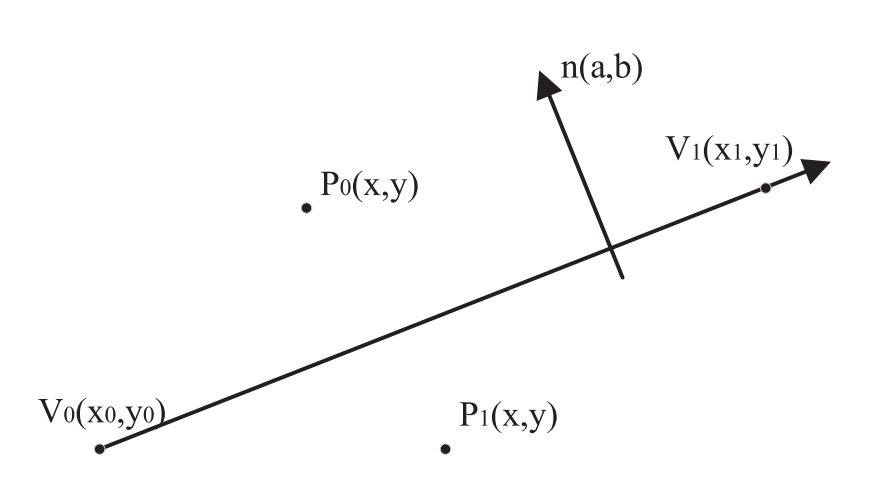
\includegraphics[width=.5\textwidth]{figure/edgefunction.png}
        \label{fig:edge funtion}
    }
    \subfloat[b][边界方程法示意图]{
        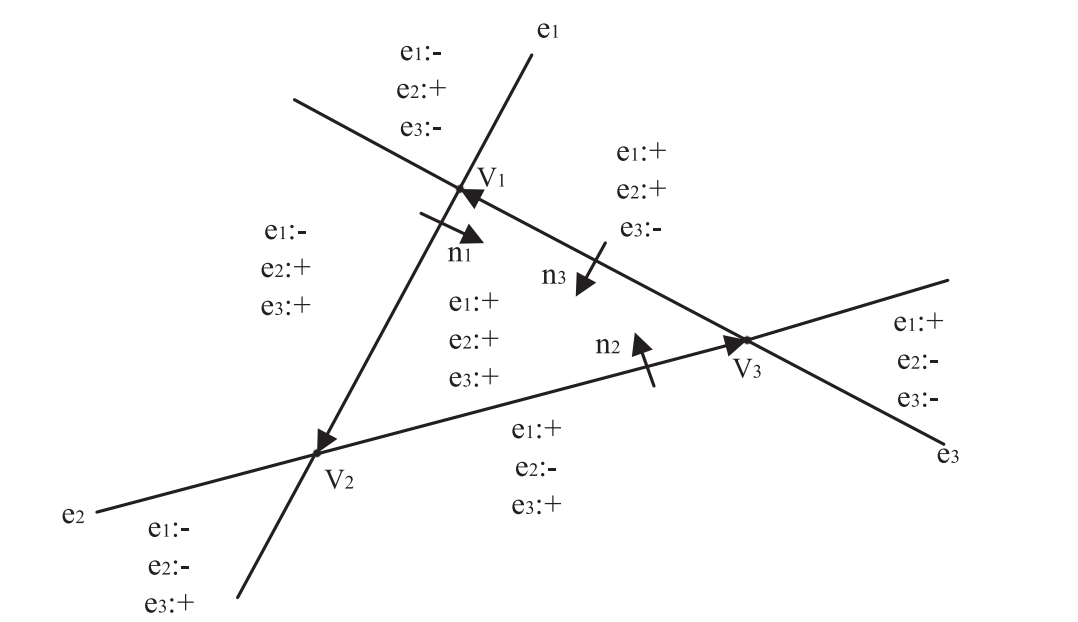
\includegraphics[width=.5\textwidth]{figure/edgefunction_1.png}
        \label{fig:edge funtion principle}
    }
    \caption{\label{fig:edge function ab}边界方程法原理}
\end{figure}
图\ref{fig:edge funtion principle}所示是edge function(边界方程)的示意图,这是一种常用的point-in-triangle测试算法,该算法的核心思想是对屏幕空间内的像素进行遍历,分别判断像素点与各顶点连线与该顶点所连的边的叉积的符号,若与三边所成叉积同号,则说明点在三角形内。具体来说,如图\ref{fig:edge funtion}所示,$\overrightarrow{V_0P_0}$与$\overrightarrow{V_0V_1}$分别是任一点与顶点的连线向量和顶点所在边的向量,这两个向量所成的叉积显示了这个点在这个边的某一侧,例如$\overrightarrow{V_0P_0}\times \overrightarrow{V_0V_1} > 0$,那么取边另一侧一点$P_1$有$\overrightarrow{V_0P_1}\times \overrightarrow{V_0V_1} < 0$。



边界方程法的整体原理显示如图\ref{fig:edge funtion principle},在图\ref{fig:edge funtion principle}中,利用图\ref{fig:edge funtion}所示的算法,可以计算出对于一个三角形来说各区域的叉积符号情况。





算法的实现见附录\ref{code:edge function}

\end{enumerate}

以上三种算法的并行性分析如下:

\begin{enumerate}
\item 面积法的并行性
    在面积法中,如图\ref{fig:square topo}判断点在三角形内需要先做叉乘求三个子三角形的面积和大三角形的面积,然后在比较子三角形面积的和与大三角形的面积。
    
    \begin{figure}[hb]
        \centering
        \subfloat[b][面积法]{
            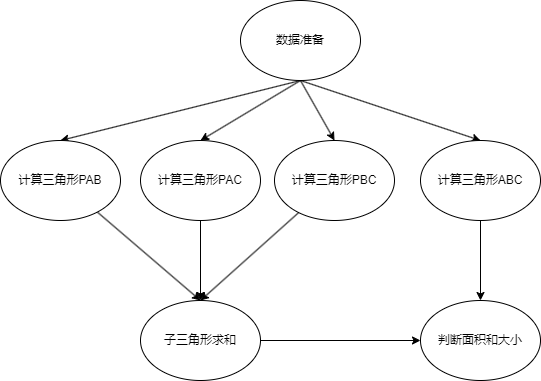
\includegraphics[width=.33\textwidth]{figure/square_topo.png}
            \label{fig:square topo}
        }
        \subfloat[b][射线法]{
            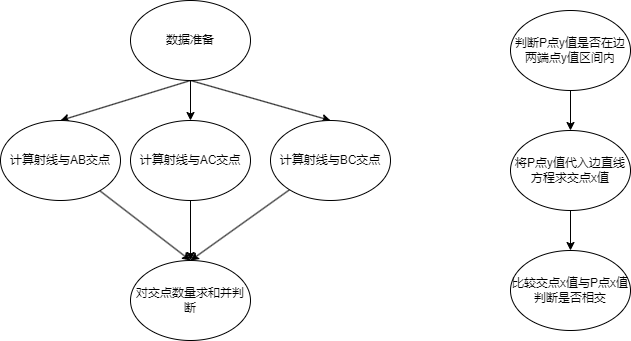
\includegraphics[width=.33\textwidth]{figure/ray_topo.png}
            \label{fig:ray topo}
        }
        \subfloat[b][边界方程法]{
            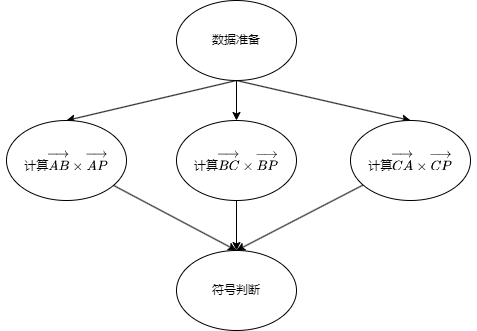
\includegraphics[width=.33\textwidth]{figure/edgefunction_topo.png}
            \label{fig:edgefunction topo}
        }
        \caption{面积法,射线法,边界方程法的拓扑结构}
    \end{figure}
    
    可以发现在面积法中,对四个三角形面积的计算可以并行来做,然后求和以及面积的比较则是串行来做。
    
\item 边界方程法的并行性
    

    类似面积法,我们可以分析图\ref{fig:edgefunction topo}所示的边界方程法拓扑结构,我们可以发现在边界方程法中,对三边的叉积计算是可以并行的,然后进行符号判断。这里和面积法比较,不但并行的开销减小,而且串行的运算也只有最后的符号判断,所以边界方程法的并行性能是优于面积法的。
    
    
\item 射线法的并行性
    
    射线法的拓扑结构是与边界方程法类似的,然而区别是边界方程法中并行的部分是三次叉积运算,而射线法并行的部分是三次射线求交点的操作。图\ref{fig:ray topo}中右侧拓扑结构为射线与三角形一边求交点的流程,相比于叉积运算,射线与边求交操作相对复杂,并且求射线与边的交点时设计计算边的斜率,即涉及浮点数的除法,计算复杂且数据稳定性较差,容易引起误差。因此判断射线法的并行不如边界方程法。
    

    
\end{enumerate}

本文将以基础的点在三角形内测试算法为出发点,设计具有高并行性的,可应用于国产GPU的点在三角形内测试系统。





\subsection{基于Cmodel的算法模型}

\subsubsection{Cmodel的定义}
在硬件设计领域,Cmodel 硬件模型通常是指使用 C 语言编写的硬件描述语言(HDL)模型。这些模型用于描述硬件功能和行为,并且可以在仿真器中进行仿真,以验证设计的正确性、功能性和性能。

使用 C 语言编写硬件模型的优点之一是,C 语言是一种相对容易学习和使用的高级编程语言,因此可以吸引更多的软件开发人员参与硬件设计。此外,C 语言的抽象级别比常见的硬件描述语言(如 Verilog 和 VHDL)更高,因此可以更快地原型设计并进行调试。

\subsection{本项目使用Cmodel的原因}

本课题的重点在于研究具有高度并行性的点在三角形内测试算法,在实验的过程中,笔者发现,在CPU上难以以多线程的方式模拟出GPU的并行效果:

为了验证中对算法进行的优化,我使用附录\ref{code:test}中的测试算法比较三种算法对单个点运算的效率。

并且使用附录\ref{code:test parallel version}中的代码对节\ref{subsubsection:analysis}中的提到的三种算法的并行性优化进行实现。

进行测试分别得到如表\ref{tab:test result}的测试结果。

\begin{table}[ht]
    \caption{\label{tab:test result}三种算法的并行性测试结果}
    \begin{tabularx}{\linewidth}{|XXX|}
        \hline
        算法 & 串行运行时长(ms) & 并行运行时长(ms) \\ \hline
        面积法 & $4.999 \times 10^{-5}$ & $1.4 \times 10^{-3}$ \\ \hline
        射线法 & $2.472 \times 10^{-5}$ & $1.0 \times 10^{-3}$  \\ \hline
        边界方程法 & $2.036 \times 10^{-5}$ & $1.1 \times 10^{-3}$  \\ \hline
    \end{tabularx}
\end{table}


可以看出开启并行优化后的运行效率反而有了数量级的退化,这在理论情况下是不可能发生的,参考GNU 14.1文档,在C++中,使用std::execution::par策略实现并行的底层原理是创建一个线程池供并行调度\cite{GNUdoc},本质上这些线程仍然要经过操作系统的调度,存在线程调度的额外开销,在算法执行速度本身很快的情况下,使用多线程反而是一种负优化。因此,后续笔者需要寻找新的并行化性能测试策略以避免这种由于模拟引起的误差。

本课题的重点在于发掘点在三角形内测试算法的并行性能,而多线程的方式必然会引入与课题算法无关的,由操作系统调度引起的误差。

所以本课题采用Cmodel的方式模拟并行算法。

\subsection{冲突可串行化}
如果要编写串行的Cmodel程序模拟并行的GPU算法,我们首先要保证并行的算法在串行执行时结果不会改变,在这里,本文使用了冲突可串行化策略。

冲突可串行化是是数据库系统中常用的概念,指的是数据库系统在多个事务并发时能够串行执行得到正确的结果,在Cmodel模拟并行的GPU时,也可以采用相同的思想,即处理并行的运算的依赖关系。

假如我们要串行模拟两个不存在依赖关系的并行运行的线程1和2,线程1需要依次执行Func A1,Func B1,Func C1,Func D1,而线程2需要依次执行Func A2,Func B2,Func C2,Func D2,我们可以发现,只要使得Func A1,Func B1,Func C1,Func D1,Func A2,Func B2,Func C2,Func D2在串行中的顺序与其在原线程中的其他函数相对位置不变,那么串行运行的结果一定和并行一致。
\begin{figure}[h]
    \centering
    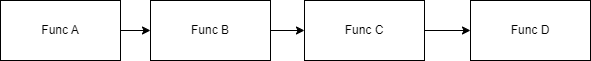
\includegraphics[width=.5\textwidth]{figure/threadtopo.png}
    \caption{线程中的执行顺序拓扑图}
    \label{fig:thread topo}
\end{figure}
\begin{figure}[ht]
    \centering
    \subfloat[b][顺序1]{
        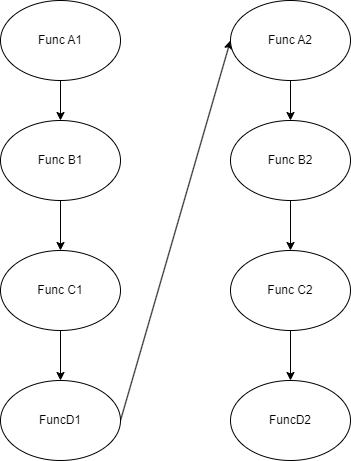
\includegraphics[width=.2\linewidth]{figure/sequnce1.png}
    }
    \subfloat[b][顺序2]{
        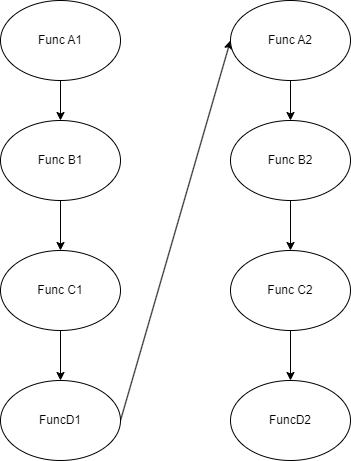
\includegraphics[width=.2\linewidth]{figure/sequnce1.png}
    }
    \subfloat[b][顺序3]{
        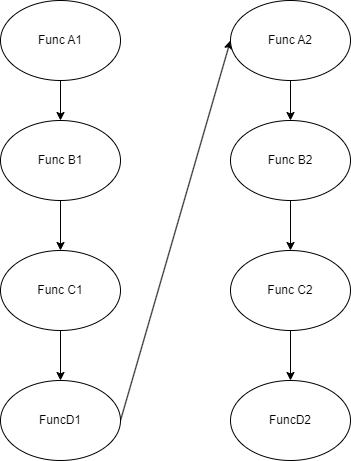
\includegraphics[width=.2\linewidth]{figure/sequnce1.png}
    }
    \subfloat[b][顺序4]{
        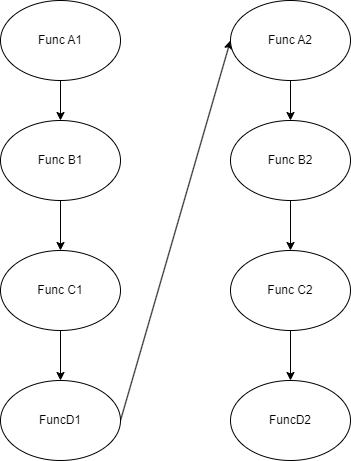
\includegraphics[width=.2\linewidth]{figure/sequnce1.png}
    }
    \caption{四种串行执行线程1,2的顺序}
    \label{fig:sequences}
\end{figure}




如图\ref{fig:sequences},序列一,二,三的执行顺序都不会影响最终运行结果的正确性,但是序列四的运行顺序是错误的,因为原本thread \ 2中的Func \ C2和Func \ B2的执行顺序颠倒了,这个序列是一个不可并行的序列。

事实上我们可以认为一个线程中顺次执行的操作为一个线性的依赖关系图,如图\ref{fig:thread topo},图中箭头表示依赖关系的方向,被箭头指向的节点视为存在依赖关系,只要我们串行执行时,每次先执行不存在依赖关系的任务,即在该拓扑图中入度为0的节点。

\begin{figure}[hb]
    \centering
    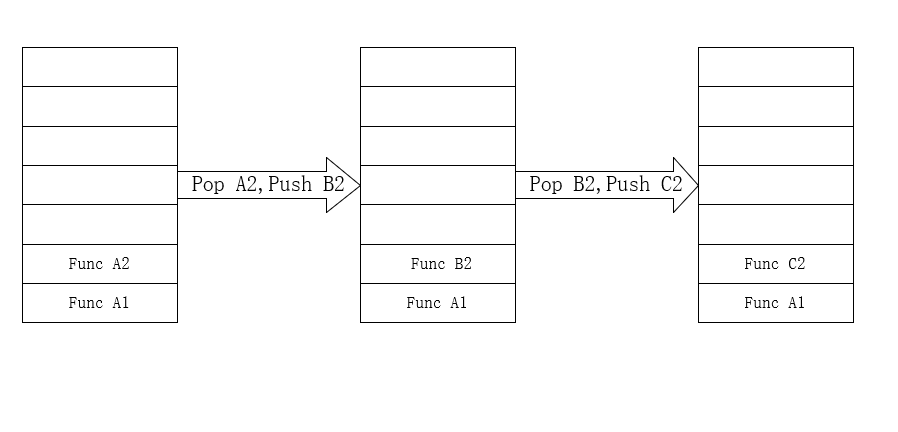
\includegraphics[width=.7\textwidth]{figure/stack.png}
    \caption{可执行任务的栈}
    \label{fig:in degree = 0}
\end{figure}

如图\ref{fig:in degree = 0}所示,我们将入度为0的节点维护成一个栈,取出栈顶节点进行处理后,产生了新的入度为0的节点,再填入栈中,我们就可以得到一个冲突可串行化的序列。整体流程如图\ref{fig:sequence gen}所示。



\subsection{时序模拟}

\subsubsection{时钟驱动}
本课题采用时钟驱动的方式编写Cmodel,具体做法为在系统中维护了一个clock,子系统的运行方式为在一个循环中不断更新clock,然后分别用更新的clock驱动子模块,如伪代码\ref{algorithm:clock}中所示。

\begin{algorithm} 
	\caption{时钟驱动的串行系统} 
	\label{algorithm:clock} 
	\begin{algorithmic}
        \STATE $Initialization:clock \gets 0$
        \WHILE{$True$}
            \STATE $module_1.clock \gets clock$
            \STATE $module_2.clock \gets clock$
            \STATE $module_3.clock \gets clock$
            \STATE $mudule_1 \ run  \ cycle$
            \STATE $module_2 \ run \ cycle$
            \STATE $module_3 \ run \  cycle$
            \STATE $clock \gets clock +1$
        \ENDWHILE
	\end{algorithmic} 
\end{algorithm}

伪代码\ref{algorithm:clock}在逻辑上相当于$module_1$,$module_2$,$module_3$共用时钟信号,并且在时钟上升沿时更新数据。

\subsubsection{延迟单元}

在有了时钟同步的基础上,我们可以将Cmodel编写的像数字电路一样,但是在Cmodel中,程序的执行并非像RTL(寄存器传输级硬件描述)中每个时钟节拍结束后才有数据的更新,为了使得Cmodel程序的运行能够模拟RTL,本课题引入了延迟单元(Latency Unit)。
\begin{figure}[h]
    \centering
    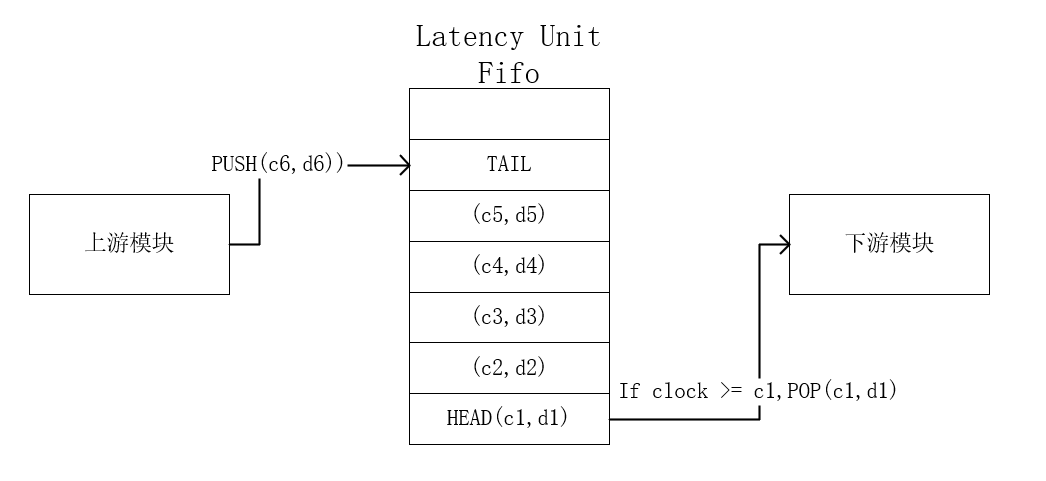
\includegraphics[width=.5\textwidth]{figure/latencyunitfifo.png}
    \caption{\label{fig:latency unit fifo}延迟单元队列工作示意图}
\end{figure}
假设Cmodel中某个上游模块在时钟为$c$时产生的数据为$d$,那么这个数据对应的Latency Unit就是数据对$(c,d)$,上游模块将数据对$(c,d)$传入下游模块的缓冲区,而下游模块要想取得数据$d$,只能等到时钟$c$时才能将d从数据块中取出,这样的设计使得上游模块只要知道数据产生的周期,将Latency Unit向下游传递,就可以保证数据产生的周期和RTL一致,也就是模拟了硬件的时序关系。延迟工作单元队列的工作流程如图\ref{fig:latency unit fifo}所示。

这样做的好处也有让Cmodel加速运行,提升模拟的效率,因为Cmodel在有了latency unit后不必严格等待每个时钟周期来运行一拍的操作,而是一次性执行多拍的操作,发送到latency unit的队列中。






\section{系统设计}

根据\nameref{subsubsection:analysis}中的讨论,本课题认为射线法和边界方程法的并行性能更优。但射线法在数值计算的角度与边界方程法有差距。

乘法和除法在数值计算中引入误差的主要原因是浮点数的有限精度。浮点数是用有限位数的二进制表示的,因此无法准确表示所有的实数。这导致在进行乘法和除法运算时,结果可能会产生舍入误差或截断误差。

\begin{equation}
    \label{eq:numerical error}
    \begin{split}
        |e(x^*+y^*)|  \leq \varepsilon (x) +  \varepsilon (y) \\ 
        |e(x^*y^*)|  \leq |x^*|\varepsilon (y) +  |y^*| \varepsilon (x) \\ 
        |e(\frac{x^*}{y^*})| \leq |\frac{x^*}{{y^*}^2}|\varepsilon(y^*) + |\frac{y^*}{{y^*}^2}|\varepsilon(x^*)
    \end{split}
\end{equation}

记误差符号为$e$,记$x^*$和$y^*$都是含有误差的值,$\varepsilon (x^*)$和$\varepsilon (y^*)$分别是$x^*$和$y^*$的误差上界,参考\cite{na},我们可以归纳出基础运算的误差为\ref{eq:numerical error}。

可以明显看出除法是误差界是最不稳定的,受被除数的影响相对较大,在射线法的计算中,涉及除法运算,具有不稳定性,而边界方程法的计算只涉及到乘法和加法,在数值上具有更高的精度,因此本课题选用边界方程法为基础展开后面的并行策略。


\subsection{Bounding Box}

\begin{figure}[H]
    \centering
    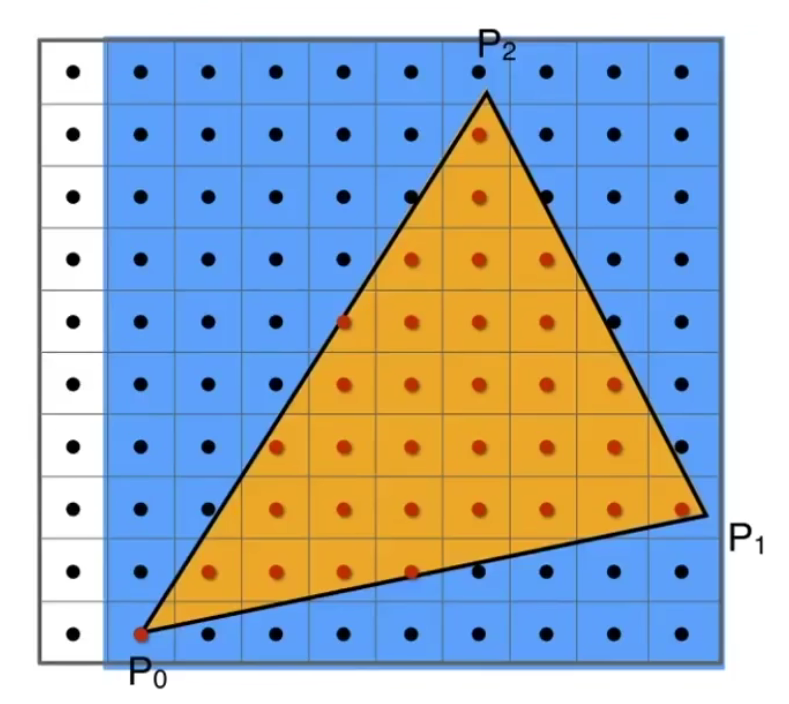
\includegraphics[width=.5\textwidth]{figure/bdbox.png}
    \caption{包围盒}
    \label{fig:bdbox}
\end{figure}

Point-in-Triangle测试算法的工作是确定屏幕空间内每个像素是否在三角形内,但事实上我们没必要对整个屏幕空间的像素进行扫描,我们可以为三角形确定一个bounding box(包围盒),这个bounding box是一个矩形,假设三角形所有顶点中,x值最大为$x_{max}$, x值最小为$x_{min}$, y值最大为$y_{max}$, y值最小为$y_{min}$, 那么包围盒四个顶点的坐标为$(x_{min},y_{min})$,$(x_{min},y_{max})$,$(x_{max},y_{min} )$,$(x_{max},y_{max})$,如图\ref{fig:bdbox}所示。在包围盒外面的像素一定不在三角形内,所以我们缩小了搜索空间,这是进行并行化优化的第一步。



\subsection{划分tile}

不论采用哪一种point-in-triangle测试算法,遍历每一个像素都是成本高昂的,显然,对于point-in-triangle算法来看,假如存在一个bounding box内的矩形,矩形的四个顶点都在三角形内,那么矩形内所有的像素都一定在三角形内,基于这一条件,我们可以在bounding box内以块的形式进行测试,为了方便对齐,我们采用$n\times n$($n$是2的幂次)规模的块进行测试,这样的块称为tile。

\subsection{tile的判断}
\label{subsubsection:tile check}
将搜索空间划分为tile的用意是减少判断的次数,对tile四个顶点的进行判断后,若四个顶点全部在三角形内,那么可以认为tile内的所有顶点都在三角形内,假设tile的规模是$32\times 32$那么判断的次数就由1024减少到了4次。

但是当四个顶点并不都在三角形内时,我们需要进行进一步的判断,如果四个顶点中存在三角形内的点,我们可以认为这个tile是有一部分在三角形内的,这时我们只能去将tile再次分割进行判断。

当四个顶点全部都不在三角形内时,我们需要判断tile是否在三角形外。考虑到tile是一个封闭图形,如果tile的四个顶点都在三角形外,那么如果tile内部有点在三角形内,那么三角形一定有至少一边穿过了tile。于是这个问题转化为了判断边是否穿过tile。

\begin{figure}[h]
    \centering
    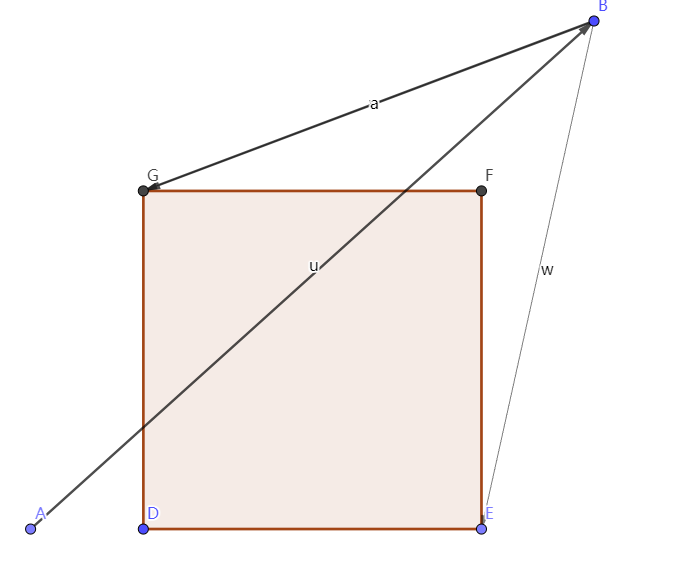
\includegraphics[width=.5\textwidth]{figure/linethroughtile.png}
    \caption{\label{fig:line tile}边穿过tile}
\end{figure}

我们可以利用图\ref{fig:edge function ab}中的原理,也是前面所利用的边界方程法的原理,向量$\overrightarrow{V_0V_1}$两侧有点$P_0,P1$,那么$\overrightarrow{V_0P_0}\times\overrightarrow{V_0V_1}$与$\overrightarrow{V_0P_1}\times\overrightarrow{V_0V_1}$一定是不同符号的,且如果$\overrightarrow{V_0P_0}\times\overrightarrow{V_0V_1}>0$,那么向量$V_0V_1$与$P_0$同侧取任意一点$P$仍然有$\overrightarrow{V_0P}\times\overrightarrow{V_0V_1}>0$。利用这个原理判断图\ref{fig:line tile}中tile的四个顶点是否在直线的两侧,只要tile四个顶点不在直线u的同侧,那么直线就一定穿过tile,反之,直线没有穿过tile。这是一个充要条件。

在实际工程中,我们判断的是三角形的边,也就是一条线段是否经过tile,只要判断这条线段的起止x,y坐标不都在tile外即可,只要满足这一点,就可以通过计算四个叉乘运算,判断三角形一边是否经过了tile。流程如图\ref{fig:line through tile flow chart}。

经过这一步判断,如果三角形有一边穿过了tile,那么我们就认为tile中有部分在三角形内,否则我们就认为这个tile中没有与三角形重合的部分,是不需要判断的无效部分。


\subsection{tile的分割}
我们首先以一个较大的tile进行搜索,通过节\ref{subsubsection:tile check}中提到的check检测方法,我们舍弃无效的tile,将三角形内的tile直接输出,剩下的部分在三角形内的tile我们进行进一步的分割。
比如原始大小为$32\times 32$的tile等分成4个$16\times 16$的后,每个子tile仍然能够应用节\ref{subsubsection:tile check}中的算法进行检测,直到tile的大小降低到一个阈值,使得我们可以一次性检测tile中的所有像素。

根据国产GPU的硬件特性,tile被分割到$2\times 2$大小即可对tile中所有像素进行并行检测。

\subsection{tile的提取}
\label{subsection:tile seek}
在屏幕空间中遍历tile的过程也可以进行优化,如果能够连续处理有效的tile,规避无效的tile能够使得测试算法的流水线保持满负载运行状态,能够提高测试算法的吞吐量,进而提升测试算法的并行性。

本课题为了保证tile提取的连续性,设计了如下算法:
\begin{enumerate}
    \item step1:\\ 初始化第一个tile的位置,左上角是三角形y方向上中间的顶点。\\ 初始化first line标志,该标志记录了算法是否扫描到了新的一行 \\ 初始化left cache,right cache,top cache,bottom cache这四个cache是记录了上下作右四个方向的缓存tile,并初始化对应的valid标志位 \\ 初始化水平扫描方向为向右,竖直扫描方向为向上
    \item step2: 判断当前tile是否有效,以及与tile相邻的四个tile是否有效
    \item step3: 如果到了新的一行,检查左侧tile是否有效,有则缓存到left cache,并置位valid标志,重置换行标志。
    \item step4: 检查上方tile是否有效,若有效且top cache valid = false,缓存上方tile,并置位valid标志
    \item step5: 检查下方tile是否有效,若有效且bottom cache valid = false,缓存上方tile,并置位valid标志
    \item step6: 判断水平扫描方向是否向右,否则跳到step12
    \item step7: 若右侧tile有效,提交当前tile,再令tile = right tile,回到step2
    \item step8:若left cache有效,取出left cache,重置left cache标志位,水平扫描方向向左,回到step2
    \item step9:判断竖直扫描方向是否为向上,否则跳到step11
    \item step10:若top cache有效,提交当前tile,取出top cache,tile = top cache,并重置top cache 的valid标志,水平扫描方向设为左,置位换行标志,回到step2。
    \item step11:若bottom cache有效,提交当前tile,取出bottom cache,tile = bottom cache,并重置bottom cache 的valid标志,水平扫描方向设为左,竖直扫描方向设为下,置位换行标志,回到step2。否则算法结束。
    \item step12:若左侧tile有效,提交当前tile,再令tile = left tile,回到step2

\end{enumerate}
\begin{figure}[H]
    \centering
    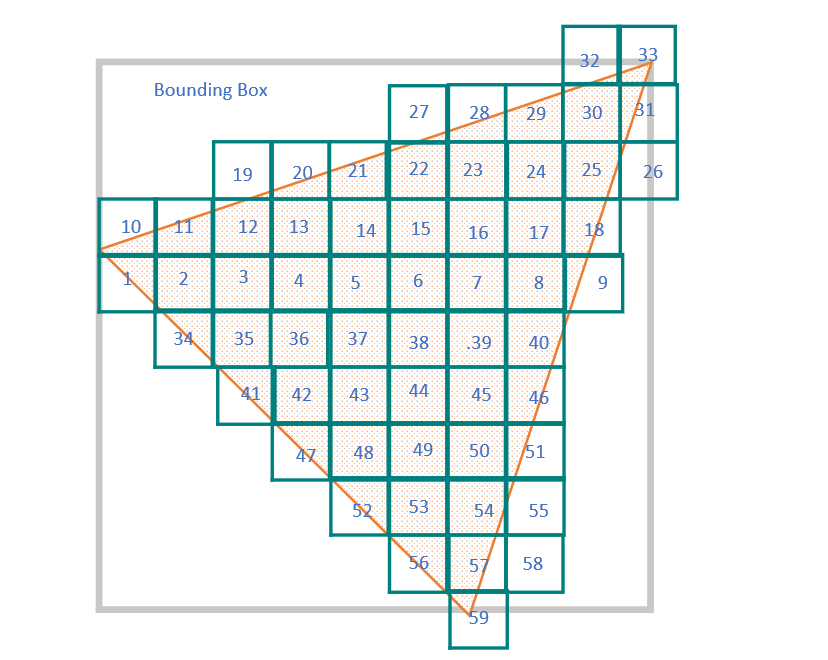
\includegraphics[width=.5\linewidth]{figure/tileorder.png}
    \caption{\label{fig:tile order in a triangle}tile扫描运行实例}
\end{figure}
算法的运行流程图如图\ref{fig:tile scan flow chart}, 图\ref{fig:tile order in a triangle}是一个例子,图中tile的标号表示在该扫描算法下tile的扫描顺序。
本节中的算法实现于源码的cTileSeeker类。






\subsection{三角形内的tile的处理}
\label{subsection:internal tile}
\begin{algorithm} [H]
	\caption{三角形内部tile的处理} 
	\label{algorithm:internal tile} 
	\begin{algorithmic}
        \STATE $Initialization:x \gets 0,y \gets 0,isCurrentTileFinished \gets false$
        \WHILE{Internal Tile Fifo is Not Empty}
            \STATE $CurrentTile \gets fifo.pop()$
            \STATE $isCurrentTileFinished \gets true$
            \STATE $x \gets CurrentTile.x$
            \STATE $y \gets CurrentTile.y$
            \WHILE{isCurrentTileFinished is false}
                \STATE $send \ 2\times 2 \ tile \  at \ (x,y)$
                \STATE $x \gets x+2$
                \IF{$x \geq CurrentTile.x + CurrentTile.size$}
                   \STATE $x \gets CurrentTile.x$
                   \STATE $y \gets y+2$
                    \IF {$Y \geq CurrentTile.Y + CurrentTile.size$}
                        \STATE $isCurrentTileFinished \gets true$
                    \ENDIF
                \ENDIF
            \ENDWHILE
        \ENDWHILE
	\end{algorithmic} 
\end{algorithm}
三角形内部tile的处理相对简单,只需要维护一个内部tile的延迟单元队列,内部tile的处理模块只要从队列中取出tile,按顺序将tile中的$2\times 2$的子tile发送到下游即刻。算法如\ref{algorithm:internal tile}所示,源码实现于类cInsideTileDecomposer。



\subsection{部分在三角形内的tile的处理}
\label{subsection:tile decompose}
\begin{algorithm} [H]
	\caption{tile分解判断} 
	\label{algorithm:tile decompose} 
	\begin{algorithmic}
        \STATE $tile \gets fifo.pop()$
        \STATE $LeftTopTile.x \gets tile.x,LeftTopTile.y \gets tile.y,LeftTopTile.size \gets tile.size/2$
        \STATE $RightTopTile.x \gets tile.x,RightTopTile.y \gets tile.y,RightTopTile.size \gets tile.size/2$
        \STATE $LeftBottomTile.x \gets tile.x,LeftBottomTile.y \gets tile.y,LeftBottomTile.size \gets tile.size/2$
        \STATE $RightBottomTile.x \gets tile.x,RightBottomTile.y \gets tile.y,RightBottomTile.size \gets tile.size/2$
        \STATE $check \ 4 \ subtile \ parallel$
        \FORALL{4 subtile}
            \STATE check tile type 
            \IF{tile is in triangle}
                \STATE send tile to internal tile module 
            \ELSIF{part of tile is in triangle} 
                \STATE send tile to next level decomposer 
            \ENDIF

            
        \ENDFOR
	\end{algorithmic} 
\end{algorithm}
如果tile有部分在三角形内,应当将tile等分成子tile,重复\nameref{subsubsection:tile check}中使用的tile检测方法,判断子tile的类型,然后发送给不同的处理模块。如果子tile在三角形内部,则发送给内部tile处理模块,如果tile部分在三角形内,则发送给下一级的内部tile处理模块。如伪代码\ref{algorithm:tile decompose}所示。



\subsection{$2\times 2$最小tile的处理}
\label{subsection:tile raster}
由于国产GPU中判断点在三角形测试的下游模块接受$2\times 2$大小的mask(mask中每一位表示$2\times 2$的tile中某一个像素是否在三角形内),所以当tile分解到大小为$2\times 2$时,我们直接并行测试tile中四个点,生成mask发送给下游即可。

\subsection{测试算法流水线}

将上述节\nameref{subsection:tile seek},\nameref{subsection:internal tile},\nameref{subsection:tile decompose},\nameref{subsection:tile raster}中设计的模块串联成测试算法的流水线如图\ref{fig:alogrithm pipeline}。


\subsection{算法运行流程可视化}

\begin{figure}[h]
    \centering
    \subfloat[b][渲染过程]{
        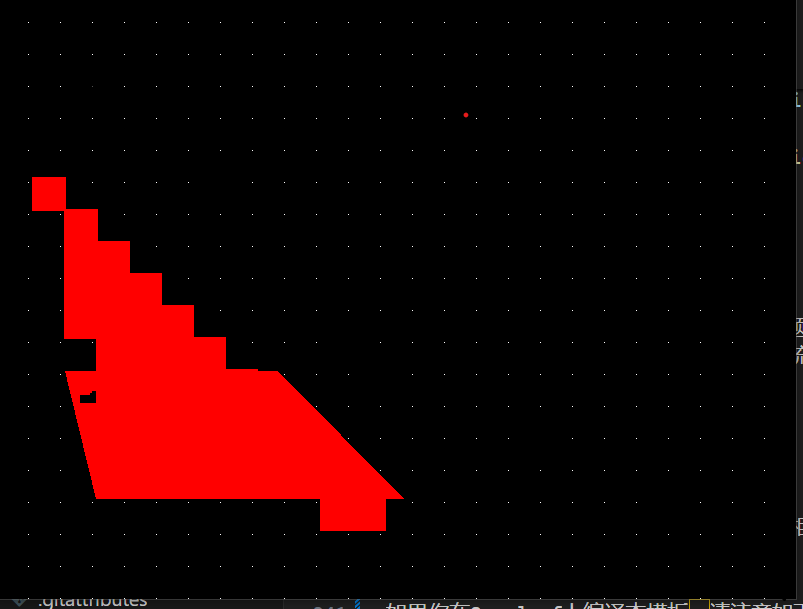
\includegraphics[width=.45\linewidth]{figure/raster1.png}    
    }
    \subfloat[b][渲染结束]{
        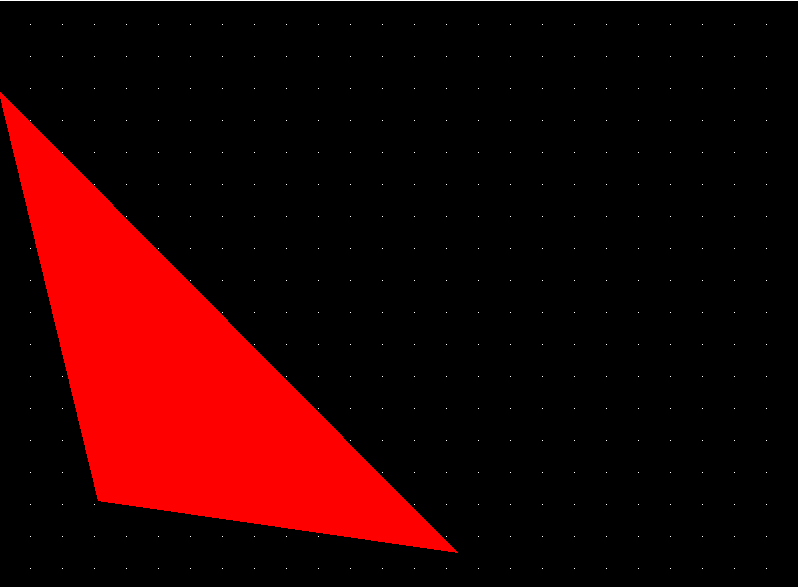
\includegraphics[width=.45\linewidth]{figure/raster2.png}
    }

    \caption{\label{fig:visualisition}算法可视化}
\end{figure}
为了方便展示算法的流水线运行过程,本课题使用了OpenGL渲染流水线输出的mask,可视化算法的运行流程,运行如图\ref{fig:visualisition}。



\section{并行分析和优化}


\subsection{边界方程法优化}
判断点P在三角形ABC内,我们需要判断P点与三条边的叉积的符号是否相同,若P在ABC内,那么P点与三边的叉积全为正或者全为负,这里的正负取决于三角形向量 $\overrightarrow{AB},\overrightarrow{BC},\overrightarrow{CA}$ 是顺时针排列还是逆时针排列。如图\ref{Fig.edgefunction_1}所示的逆时针排列时,三角形内部的叉积符号为正,反之则为负。

只要我们在输入三角形时对三角形顶点顺序进行重新排列,使得$\overrightarrow{AB},\overrightarrow{BC},\overrightarrow{CA}$ 的排列是逆时针,即可保证三角形内的叉积符号为正。分别在x和y方向(坐标系如图\ref{Fig:two triangle},原点建立在屏幕空间左上,向右和向下分别是x,y轴正方向)对顶点进行排序,\\ 令$V_{x_{min}},V_{x_{mid}},V_{x_{max}},V_{y_{min}},V_{y_{mid}},V_{y_{max}}$分别为x方向,y方向上最小值点,中点和最大值点。
只要令$A=V_{y_{min}},B=V_{y_{max}},C=V_{y_{mid}}$,若$x_C<x_B$,那么三角形的围绕方向为顺时针,叉积符号为负,反之则为正。另外保证三角形三个顶点的相对位置关系后续也可拓展实现DirectX中的top-left规则。
另外为了排除三角形出现在屏幕空间中不同位置导致的浮点数运算精度差异,我们为每个三角形选取一个相对三角形本身固定的点作为起始点,将这个起始点作为对该三角形进行测试的坐标原点。分析P点(x,y)相对于三边的叉积,记叉积符号为E,则起始点$(x,y)$相对于三角形三边的叉积如式\ref{eq:ab bc ca product of init point}。

\begin{equation}
    \label{eq:ab bc ca product of init point}
    \begin{split}
        E_{AB} (x,y)&=(x-x_A )(y_B-y_A )-(y-y_A )(x_B-x_A ) \\
        E_{BC} (x,y)&=(x-x_B )(y_C-y_B )-(y-y_B)(x_C-x_B) \\
        E_{CA} (x,y)&=(x-x_C )(y_A-y_C )-(y-y_C)(y_A-y_C)
    \end{split}
\end{equation}

对屏幕空间内其他任意一点$P$可以表示为$(x+x_{\delta},y+y_{\delta})$,记$x_{AB} = x_B-x_A,y_{AB} = y_B-y_A,x_{BC} = x_C-x_B,y_{BC} = y_C-y_B,x_{CA} = x_A-x_C,y_{CA} = y_A-y_C$,式\ref{eq:ab bc ca product of init point}可以变式为式\ref{eq:product relative to init point}

\begin{equation}
    \label{eq:product relative to init point}
    \begin{split}
        E_{AB} (x,y)&=E_{AB} (x_{init},y_{init} )+(x-x_{init} ) y_{AB}-(y-y_{init} ) x_{AB} \\
        E_{BC} (x,y)&=E_{BC} (x_{init},y_{init} )+(x-x_{init} ) y_{BC}-(y-y_{init} ) x_{BC} \\
        E_{CA} (x,y)&=E_{CA} (x_{init},y_{init} )+(x-x_{init} ) y_{CA}-(y-y_{init} ) x_{CA}
    \end{split}
\end{equation}
这样的变式并不会增加运算量,并且消除了因为点的位置引起的测试过程中的浮点误差差异。

在具体实现时,对于一个三角形的测试中,我们只需要计算一次与三角形和初始点有关的$E_{AB}(x_{init},y_{init})$,$E_{BC}(x_{init},y_{init})$,$E_{CA}(x_{init}$,$y_{init})$,
$y_{AB}$,$y_{BC}$,$y_{CA}$,$x_{AB}$,$x_{BC}$,$x_{CA}$。

每次检测新的点是否位于三角形内时,只要计算$(x-x_{init},y-y_{init})$带入式\ref{eq:product relative to init point}即可完成这一点相对于三边的叉积计算。



\subsection{模块时钟分析}
要想分析和优化算法的并行性,那么就要从算法的时序关系入手,分析时序关系,首要的就是确定算法各个环节所用的时钟周期。

\subsubsection{边界方程测试法的时钟周期}

对一点的边界方程法的测试是本测试系统中最频繁的操作,本课题中希望这个操作能够尽可能地并行化。

参考式\ref{eq:product relative to init point},以及依赖关系图\ref{fig:edgefunction topo},我们分配足够的计算单元,计算一个叉积$E_{AB}(x,y)$在数字电路中可以由两个加法器来并行计算$x-x_{init}$,$y-y_init$,分配两个乘法单元并行计算$(x-x_{init})y_{AB}$和$(y-y_{init})x_{AB}$,再分配一个减法器计算两个乘法结果的减法$(x-x_{init})y_{AB} - (y-y_{init})x_{AB}$, 最后分配一个加法器将上一步的结果加上一个$E_{AB}(x_{init},y_{init})$,总延迟是一个乘法延迟加上一个减法延迟再加上一个加法延迟。

最后判断三个叉积的结果是否同号的运算是一个与运算,因而边界方程法的算法延迟是$t_{mul}+t_{sub}+t_{add}+t_{and}$,($t_{add},t_{sub},t_{mul},t_{and}$分别是加法,减法,乘法和与门的延迟)。由于本课题使用Cmodel进行模拟,并不设计实际芯片工艺领域的具体工艺数据,因此这里的延迟计算仅仅作为参考,为了方便期间,我们认为对一点的边界方程法的测试是一个周期内完成的,是流水线周期大小的下界。

\subsubsection{判断tile的类型}

判断tile的类型的过程如图\ref{fig:tile check topo flow},根据
节\nameref{subsubsection:tile check}中的描述,判断三角形的边是否穿过tile事实上是比较三角形的边的$x,y$的范围是否与tile重合,以及tile四个顶底相对于三角形一边的叉积,事实上计算叉积已经在判断点是否在三角形中的这一步已经计算完毕,所以判断tile的类型的最长计算路径相比于测试一点是否在三角形中只是多了一个比较器延迟(约等于加法器延迟),和两个与门,一个或门,相比于判断一点是否位于三角形中使用的乘法运算(乘法器在数字电路中需要时钟同步,并做多周期运算\cite{ca}),增加的计算延迟相对来说较小,所以本课题认为判断tile类型也只需要一个时钟周期。


\subsubsection{tile提取所用的周期}

首先扫描提取tile的过程第一步是判断当前tile以及其相邻tile的状态,并行来做的话需要一个周期。

后续流程中,对left cache,bottom cache,top cache的更新可以并行进行判断和值的更新,这需要一个时钟周期。

进行判断的操作由于判断依赖的值以及是以前周期已经计算好的值,所以判断的时间忽略不计。

扫描算法找到寻找下一个tile的操作必须要在对cache更新之后,不能和tile更新进行并行,所以后续寻找下一个tile进行更新的过程需要一个周期。

因此扫描屏幕空间中提取一个tile的操作需要三个时钟周期。

\subsection{三角形内的tile}
三角形内的tile提取出mask几乎不需要任何运算,这里我们需要衡量的是一个周期输出多少个$2\times 2$个mask tile。这里暂定为1。

\subsubsection{tile分解}

对于部分在三角形内的tile,我们需要将其分解为四个子tile进行判断,进而发送给其他的处理单元,这里由于四个子tile是否需要有效是未知的,如果我们以流水线的方式判断四个子tile,也就是每周期判断一个子tile,下游可能会出现等待的现象,所以这里我们采用四个子tile并行测试的做法,避免下游出现等待现象。所以tile的分解需要一个周期。

\subsubsection{$2\times 2$tile生成mask}

这个模块会被频繁调用,因而直接并行的测试$2\times 2$tile中四个点,生成mask,只需要一个周期。


\subsection{并行性能的衡量指标}

\begin{itemize}
    \item \textbf{流水线的吞吐量}:即单位时间内,流水线处理了多少个$32\times 32$tile或者输出了多少个$2\times 2$mask,在本课题中采用的方法是处理固定数量的三角形,比较处理所用的时钟周期数量。
    \item \textbf{流水线的负载均衡情况}:评价并行系统的另一个角度是同一时间内有多少个模块在并行工作,因而我们需要统计在流水线的运行过程中,各模块的负载率(即工作的时钟周期占比),比较各模块的负载率,如果各模块负载率均衡,那么说明整体流水线各个模块的吞吐量较为一致,并行冗余较少。
\end{itemize}




\subsection{流水线中模块工作速率的差异以及缓冲区的设计}
流水线中各模块的工作速率是存在差异的,以TileSeeker到TileDecomposer的流水线为例,可能会有如下情况。

\begin{figure}[H]
    \centering
    \subfloat[b][流水线中每一级只向下一级传递一个tile]{
        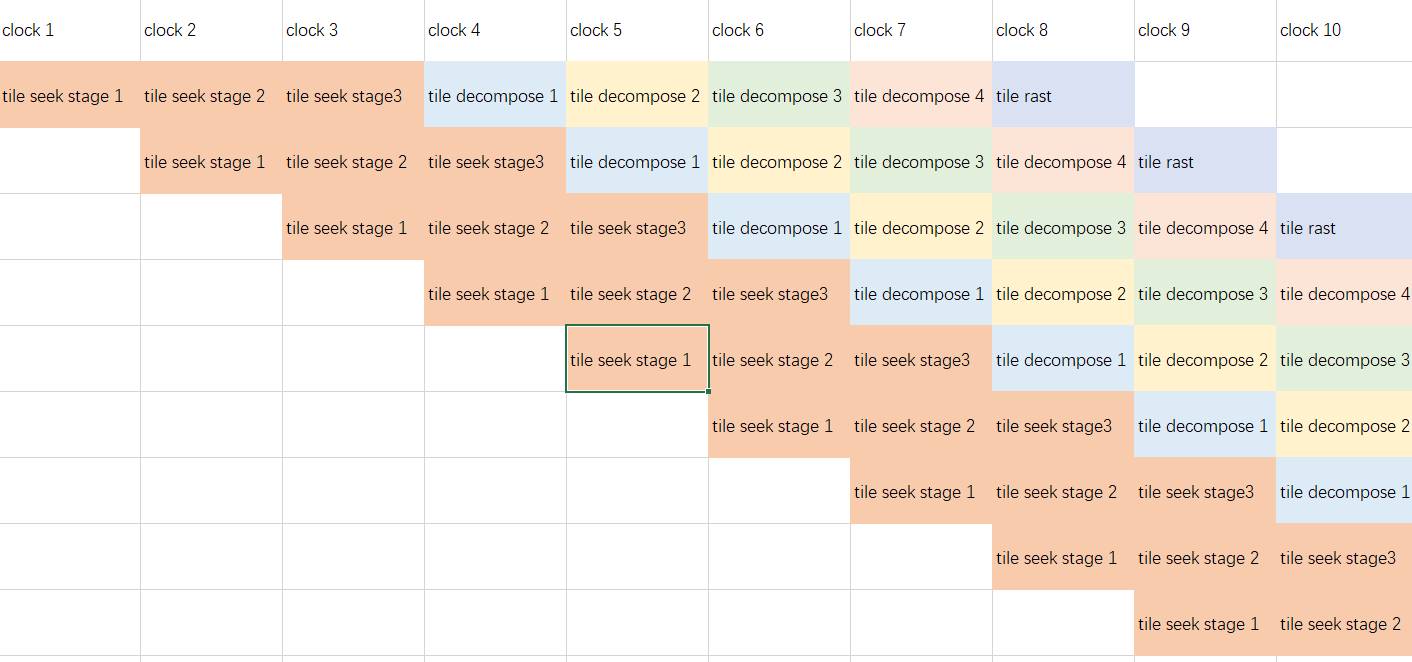
\includegraphics[width=.33\linewidth]{figure/pipeline_decompose_ideal.png}
        \label{fig:1 tile for each level}
    }
    \subfloat[b][流水线中每一级向下一级传递4个tile]{
        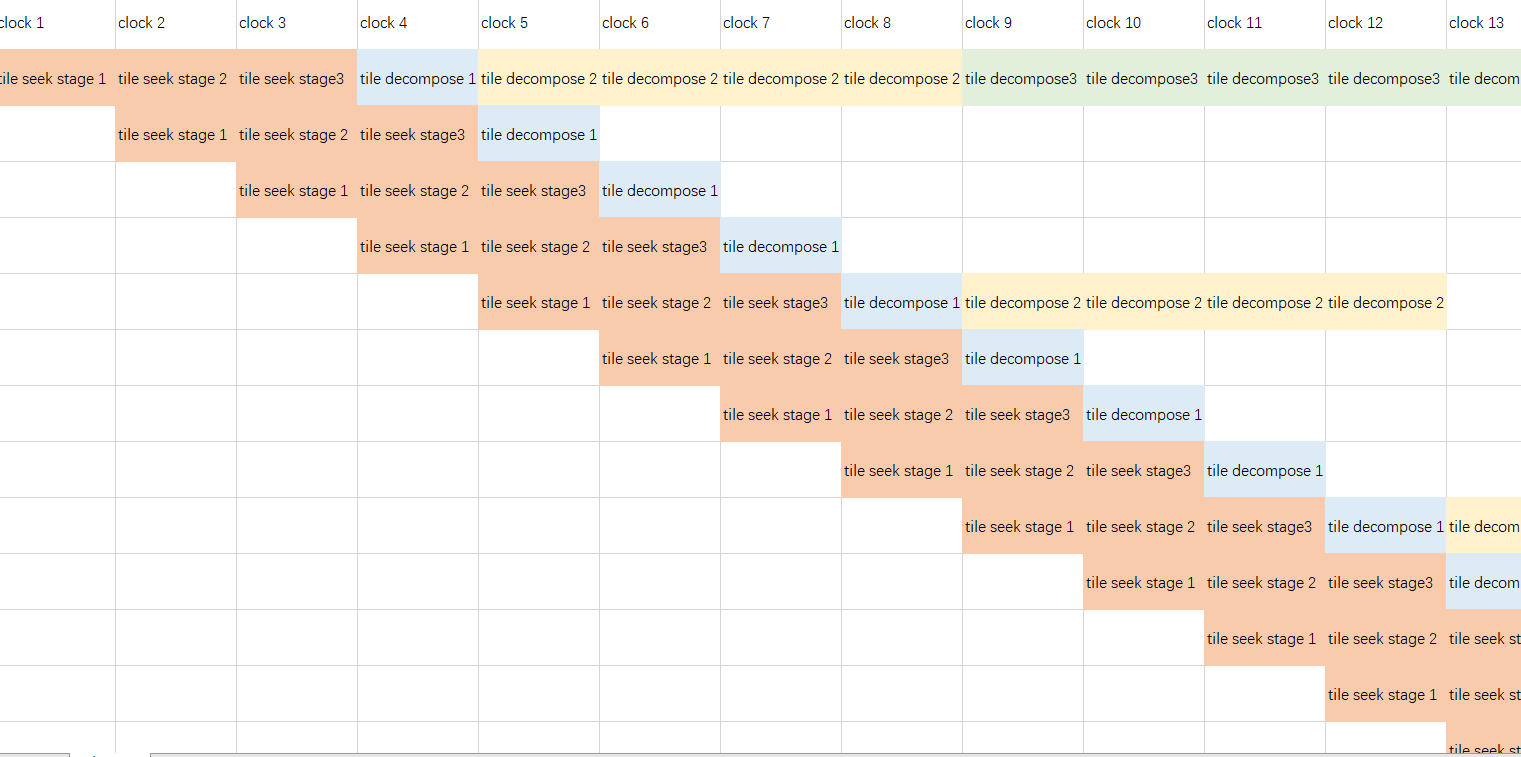
\includegraphics[width=.33\linewidth]{figure/4tileeachlevel.png}
        \label{fig:4 tile for each level}
    }
    \subfloat[b][流水线缓冲区已满]{
        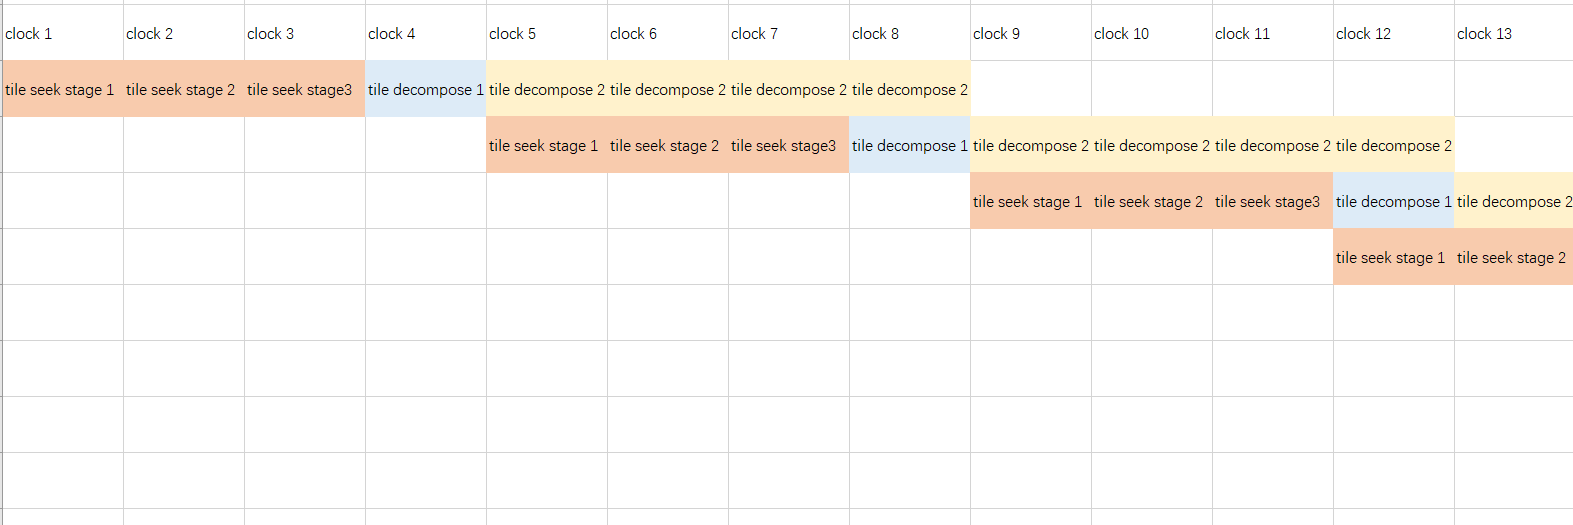
\includegraphics[width=.33\linewidth]{figure/fullbuffer.png}
        \label{fig:full buffer}
    }
    \caption{流水线运行示例}
\end{figure}
\begin{enumerate}
    \item 流水线中每一级只向下一级传递一个tile \\
    如图\ref{fig:1 tile for each level}, 进入full pipeline(流水线进入稳定状态,所有模块都在运行)状态下实际吞吐量为每周期一个$32\times 32$tile。
    \item 流水线中每一级tile decomposer向下一级decomposer传递4个tile ,如图\ref{fig:4 tile for each level},(由于流水线深度过高,这里只画到了第二级的tile decomposer)。
\end{enumerate}
在上述两种情况中,流水线模块各模块工作速度存在差异,在模块见设置缓冲区,能够平衡上述两种情况导致的流水线模块等待现象,提高并行性。
为了防止节\nameref{subsubsection:extreme}中提到的缓冲区溢出问题,流水线应当设置停止等待机制。
至于缓冲区的大小,我们参考\cite{CA}中的queuing theory,认为缓冲区的长度应当满足Little's Law\ref{eq:Little's Law},其中$L,\lambda,W$分别指队列的长度,数据包的平均到达速度和数据包在队列中的平均等待时间,这几项参数我们会在节\nameref{label:result}中进行测试。
\begin{equation}
    \label{eq:Little's Law}
    L = \lambda \cdot W
\end{equation}

\subsection{面向模块负载均衡的优化}
流水线的性能取决于流水线中的bottle neck。

为了方便找到系统流水线中的bottle neck,本课题绘制了系统运行各模块负载的甘特图,运行用例为屏幕空间宽800,高600,三角形三点为(100,100),(460,48),(0,512),绘图只取前200个时钟,结果如图\ref{fig:module gantt}。
\begin{figure}[H]
    \centering
    \subfloat[b][一周期生成1个$2\times 2$mask]{
        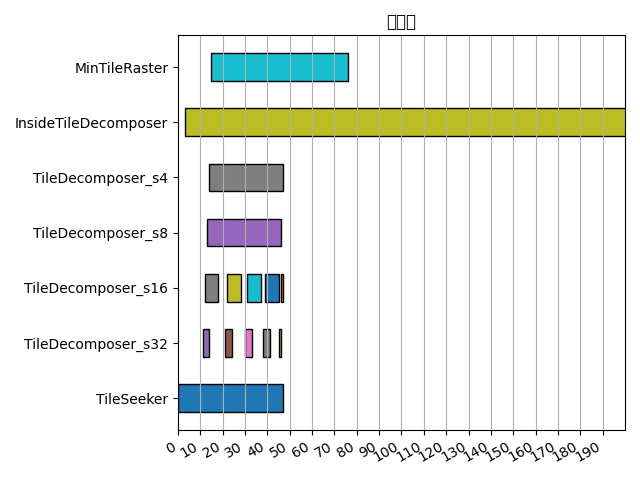
\includegraphics[width=.45\linewidth]{figure/primitiveGanttChart.png}
        \label{fig:module gantt}
    }
    \subfloat[b][一周期生成1个$2\times 2$mask]{
        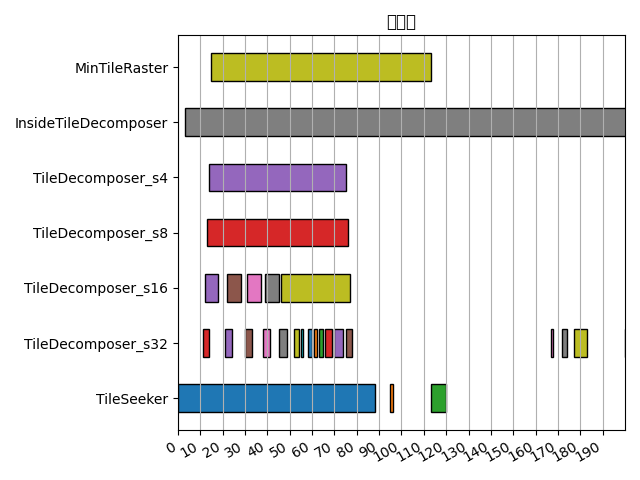
\includegraphics[width=.45\linewidth]{figure/16maskganttchart.png}
        \label{fig:16 mask gantt chart}
    }
    \caption{InsideTileDecomposer不同时系统各模块的负载情况}
\end{figure}

根据图\ref{fig:module gantt}所示,在各个模块中,负载最小的是tile decomposer,负载最大的是InsideTileDecomposer,这说明在较大的三角形的光栅化中,内部的tile数量是最多的,整个流水的瓶颈在于内部tile的处理。

\subsubsection{内部tile的优化并行处理}
由于在国产GPU下游的硬件约束中,下游可以一次性接受16个$2\times 2$mask进行一次并行处理,因此这里我们设计处理三角形内tile的模块一周期输出16个$2\times 2$mask,达到内部tile处理的最大并行性。



\begin{figure}[H]
    \centering
    \subfloat[b][较狭长的三角形]{
        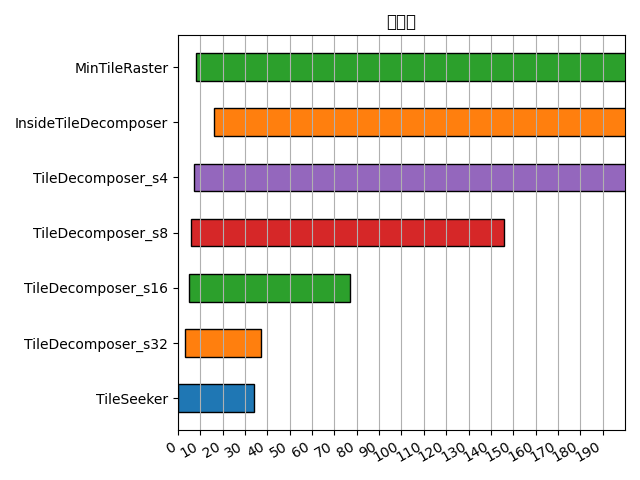
\includegraphics[width=.45\linewidth]{figure/thintriangle.png}
        \label{fig:thin triangle}
    }
    \subfloat[b][较小的三角形]{
        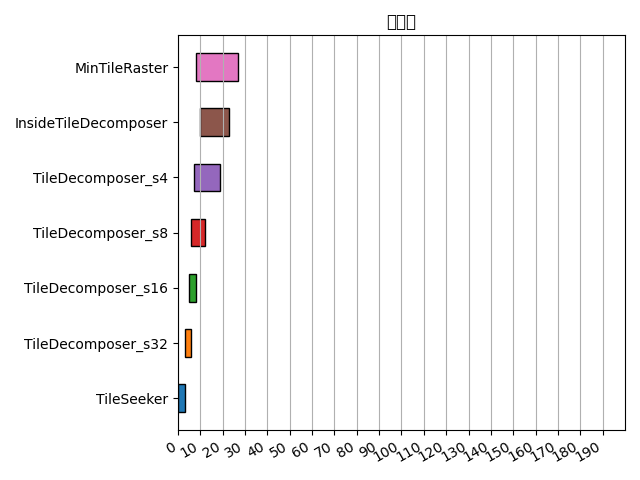
\includegraphics[width=.45\linewidth]{figure/smalltriangle.png}
        \label{fig:small triangle}
    }
    \caption{较狭长的三角形和较小的三角形下算法的算法运行负载}
\end{figure}

增加InsideTileDecomposer的并行处理能力后,模块运行的甘特图如图\ref{fig:16 mask gantt chart}所示,从图上可以看出来,InsideTileDecomposer仍然是bottleneck,然而这样的甘特图形状和测试用例的选取有关,\ref{fig:16 mask gantt chart}中的三角形较大,三角形内部的tile较多,因而InsideTileDecomposer的处理压力最大,为了避免数据偏差,我们应当测试系统在对较小三角形(三点为(100,100),(120, 110),(110,115))和较狭长的三角形(三点为(100,100),(700,120),(350,130))做测试,如图\ref{fig:thin triangle}和\ref{fig:small triangle}所示。

使用源码resource文件下的RandomTriangleList.txt中的100个随机三角形进行测试,得到的数据如表\ref{tab:100 random triangles}:

\begin{table}[ht]
    \caption{\label{tab:100 random triangles}100个随机三角形下的算法系统负载}
    \begin{tabularx}{\linewidth}{|XXX|}
        \hline
        模块 & 运行周期 & 负载率(\%) \\ \hline
        所有模块 & 70538 & 100 \\ \hline
        Tile Seeker & 3645 & 5.2  \\ \hline
        Tile Decomposer 32 & 2910 & 4.1  \\ \hline
        Tile Decomposer 16 & 5953 & 8.4  \\ \hline
        Tile Decomposer 8 & 11828 & 17  \\ \hline
        Tile Decomposer 4 & 21553 & 31  \\ \hline
        Inside Tile Decomposer & 68839 & 98 \\ \hline
        Minumum Tile Raster & 32496 & 46 \\ \hline
    \end{tabularx}
\end{table}




可以发现InsideTileDecomposer仍然是流水线中的性能瓶颈,我们进一步考虑,InsideTileDecomposer的工作方式是每个周期根据接收到的tile对应地生成16个$2\times 2$mask,这种工作方式用16个周期处理一个$32\times 32$tile,4个周期处理一个$16\times 16$tile,1个周期处理一个$8\times 8$tile,然而在处理$4\times 4$tile和$2\times 2$tile时也要消耗掉一个时钟周期,而系统流水线生成的$4\times 4$tile和$2\times 2$tile数量是相当多的,因此本课题对此进行了优化:设计$4\times 4$tile buffer和$2\times 2$tile buffer。
当模块接受tile时,若大小为2或4,存入$4\times 4$tile buffer和$2\times 2$tile buffer,模块每个周期的运行流程如伪代码\ref{algorithm:Inside Tile Decomposer with tile accumulating}所示。

\begin{algorithm} 
	\caption{Inside Tile Decomposer with tile accumulating} 
	\label{algorithm:Inside Tile Decomposer with tile accumulating} 
	\begin{algorithmic}
    \IF{Current Tile Finished}
        \IF{$2\times 2$tile buffer' size $\geq$ 16}
            \STATE generate 16 mask from $2\times 2$tile buffer and clear buffer
            \STATE go next clock
        \ELSIF{$4\times 4$tile buffer's size $\geq$ 4}
            \STATE generate 16 mask tiles from $4\times 4$tile buffer and clear buffer
        \ELSE
            \IF{orther size tile buffer is not empty}
                \STATE pop a tile from buffer 
                \STATE $isCurrentTileFinished \gets false$
            \ELSE 
                \STATE go next clock
            \ENDIF
        \ENDIF
    \ELSE 
        \STATE generate 16 mask tiles from current tile
        \STATE go next clock
    \ENDIF
	\end{algorithmic} 
\end{algorithm}

优化后在100个随机三角形的数据集运行情况如表\ref{tab:100 random triangles with improved inside decomposer},可以看出整体性能提升了30.44\%。
\begin{table}[ht]
    \caption{\label{tab:100 random triangles with improved inside decomposer}100个随机三角形下的算法系统负载}
    \begin{tabularx}{\linewidth}{|XXX|}
        \hline
        模块 & 运行周期 & 负载率(\%) \\ \hline
        所有模块 & 49063 & 100 \\ \hline
        Tile Seeker & 3645 & 5.2  \\ \hline
        Tile Decomposer 32 & 2910 & 4.1  \\ \hline
        Tile Decomposer 16 & 5953 & 8.4  \\ \hline
        Tile Decomposer 8 & 11828 & 17  \\ \hline
        Tile Decomposer 4 & 21553 & 31  \\ \hline
        Inside Tile Decomposer & 37789 & 77 \\ \hline
        Minumum Tile Raster & 32496 & 66 \\ \hline
    \end{tabularx}
\end{table}

\subsubsection{tile decomposer的动态调度优化}
\begin{figure}[H]
    \centering
    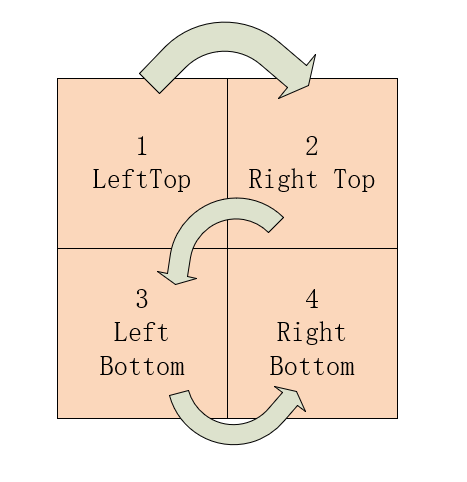
\includegraphics[width=.5\linewidth]{figure/decomposeunit.png}
    \caption{\label{fig:sub quad check order}Decomposer Unit检测子tile的顺序}
\end{figure}
根据表\ref{tab:100 random triangles with improved inside decomposer}的数据,目前tile seeker和tile decomposer的利用率非常低,考虑到tile decomposer的多级流水线机制中每一级使用了相同的运算逻辑,因此我们可以考虑使用动态调度的做法,复用相同的计算器件,具体设计上,本课题设计了一种Decomposer Unit, Decomposer Unit事实上是将原来的每一级Tile Decomposer的串行版本,Decomposer Unit接受到tile后分四个周期串行判断tile的四个子tile。子tile的判断顺序如图\ref{fig:sub quad check order}。Decomposer Unit维护了一个提交队列和一个输入缓存队列,每个周期从输入缓存中取出tile,每周期顺次判断四个子tile,每周期将判断的结果放入提交队列中,每周期提交队列向外部输出一个tile。算法流程如伪代码\ref{algorithm:decomposer unit}所示。



\begin{algorithm}
\caption{\label{algorithm:decomposer unit}decomposer unit的运行逻辑}
    \begin{algorithmic}
        \STATE initialization:$isCurrentTileFinished \gets true$ 
        \STATE initialization: $QuadId \gets 0$
        \IF{commit queue is not empty}
            \STATE $tile \gets CommitQueue.Front$
            \IF{this tile can be committed}
                    \STATE commit tile
                    \STATE commit queue pops one tile
            \ENDIF 
        \ENDIF

        \IF{commit queue is full}
            \STATE go next clock
        \ENDIF

        \IF{isCurrentTileFinished is true}
            \IF{input tile buffer is empty}
                \STATE go next clock
            \ELSE
                \STATE $CurrentTile \gets InputTileBuffer.pop$
                \STATE $isCurrentTileFinished \gets false$
            \ENDIF
        \ENDIF

        \IF{QuadId equals 0}
            \STATE check LeftTop Tile and commit to queue
            \STATE $QuadId \gets QuadId + 1$
            \STATE go next clock
        \ELSIF{QuadId equals 1}
            \STATE check RightTop Tile and commit to queue
            \STATE $QuadId \gets QuadId + 1$
            \STATE go next clock
        \ELSIF{QuadId equals 2}
            \STATE check LeftBottom Tile and commit to queue
            \STATE $QuadId \gets QuadId + 1$
            \STATE go next clock
        \ELSIF{QuadId equals 3}
            \STATE check RightBottom Tile and commit to queue
            \STATE $QuadId \gets 0$
            \STATE $isCurrentTileFinished \gets true$
            \STATE go next clock
        \ENDIF
        
    \end{algorithmic}
\end{algorithm}

动态调度策略为每个周期按x4TileFifo,x8TileFifo,x16TileFifo,x32TileFifo的优先级提取出四个tile,分别放入四个最空闲的Decomposer Unit(这里认为Decomposer Unit的输入tile缓存空闲空间越大,单元越空闲)。

在这种调度策略下,只需要8个Decomposer Unit即可达到原本静态的四级流水的性能(所用的并行资源相当于16个Decomposer Unit)。测试结果如表\ref{tab:100 random triangles with 8 decomposer unit}。


\begin{table}[ht]
    \caption{\label{tab:100 random triangles with 8 decomposer unit}应用8个Decomposer Unit在100个随机三角形测试机中的负载}
    \begin{tabularx}{\linewidth}{|XXX|}
        \hline
        模块 & 运行周期 & 负载率(\%) \\ \hline
        所有模块 & 48589 & 100 \\ \hline
        Tile Seeker & 3645 & 7.5  \\ \hline
        Decomposer Unit 0 & 27604 & 57  \\ \hline
        Decomposer Unit 1 & 24428 & 50  \\ \hline
        Decomposer Unit 2 & 21892 & 45  \\ \hline
        Decomposer Unit 3 & 20412 & 42  \\ \hline
        Decomposer Unit 4 & 19364 & 40  \\ \hline
        Decomposer Unit 5 & 18848 & 39  \\ \hline
        Decomposer Unit 6 & 18428 & 38  \\ \hline
        Decomposer Unit 7 & 18000 & 37  \\ \hline
        Inside Tile Decomposer & 37741 & 78 \\ \hline
        Minumum Tile Raster & 32496 & 67 \\ \hline
    \end{tabularx}
\end{table}

\subsection{mask输出的优先级}
在我们的系统中有Inside Tile Decomposer和Minimum Tile Raster 生成mask tile,而系统下游一周期只能处理16个$2\times 2$mask,因此在有限的信道下,为了保证每周期下输出信道是饱和的,以及Inside Tile Decomposer的吞吐量,我们有限从Inside Tile Decomposer的输出缓存中输出mask(在我们的算法模式下,三角形内部的tile占多数,Minmum Tile Raster处理的往往是三角形的边界部分),当Inside Tile Decomposer输出缓存清空时我们再输出由Minimum Tile Raster产生的mask。

如果处理的三角形较为狭长或者较小,这种工作模式可能不是最优的,但是根据算法在随机三角形测试集的表现,我们认为Inside Tile Decomposer在普遍情况下应该具有更高优先级。


\section{测试结果与分析}
\label{section:result}
\subsection{正确性验证}
\begin{figure}[H]
    \centering 
    \subfloat{
        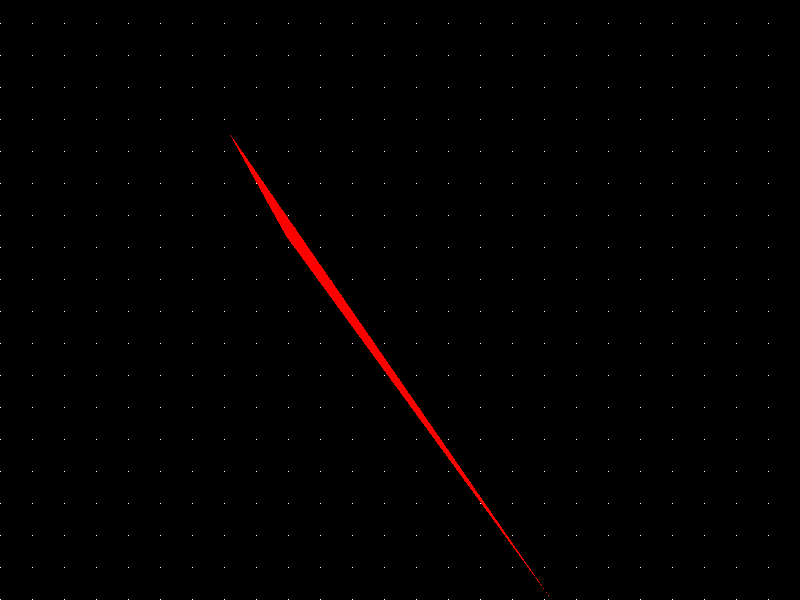
\includegraphics[width=.3\linewidth,bb = 0 0 30cm 30cm]{figure/Result0.png}
    }
    \subfloat{
        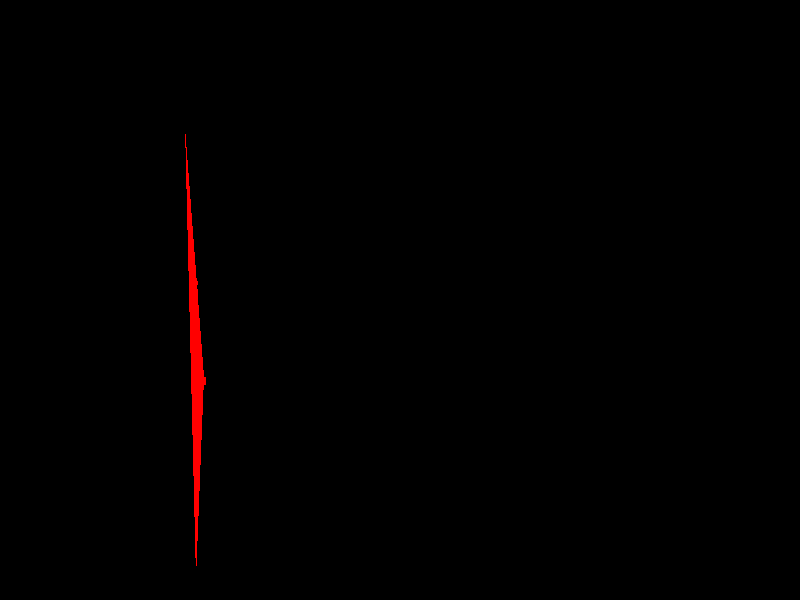
\includegraphics[width=.3\linewidth,bb = 0 0 30cm 30cm]{figure/Result1.png}
    }
    \subfloat{
        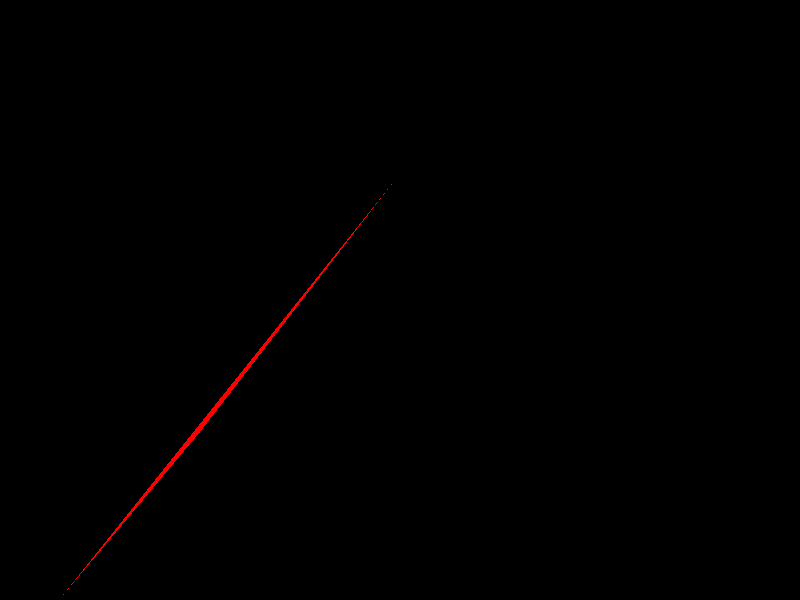
\includegraphics[width=.3\linewidth,bb = 0 0 30cm 30cm]{figure/Result2.png}
    }
    \\
    \subfloat{
        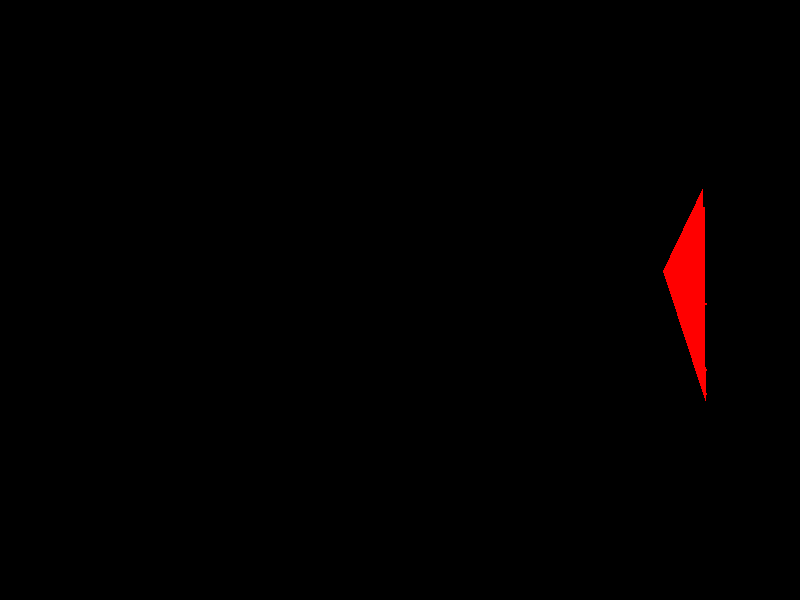
\includegraphics[width=.3\linewidth,bb = 0 0 30cm 30cm]{figure/Result3.png}
    }
    \subfloat{
        
\includegraphics[width=.3\linewidth,bb = 0 0 30cm 30cm]{figure/Result4.png}
    }
    \subfloat{
        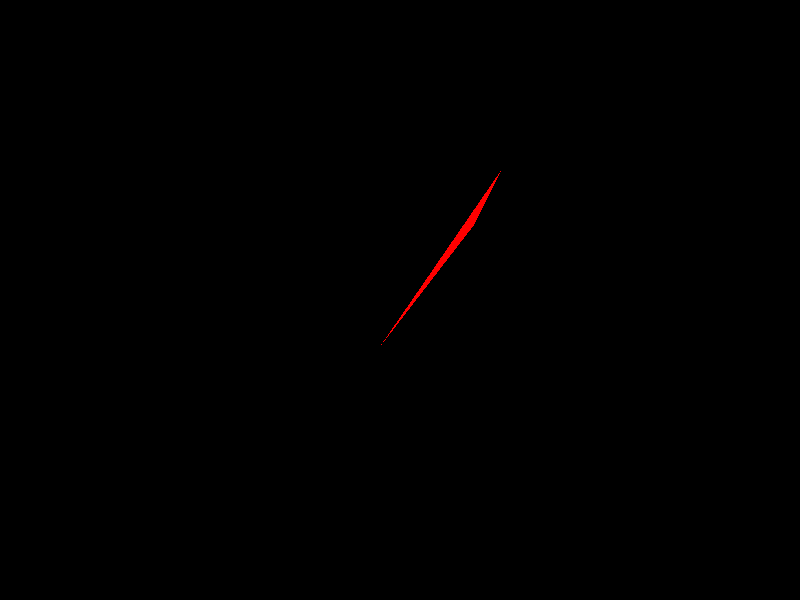
\includegraphics[width=.3\linewidth,bb = 0 0 30cm 30cm]{figure/Result5.png}
    }
    \\
    \subfloat{
        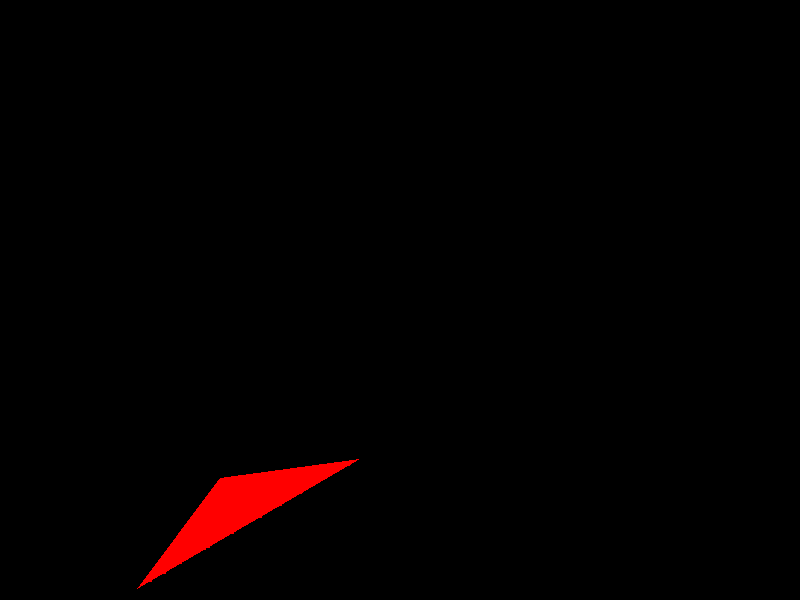
\includegraphics[width=.3\linewidth,bb = 0 0 30cm 30cm]{figure/Result6.png}
    }
    \subfloat{
        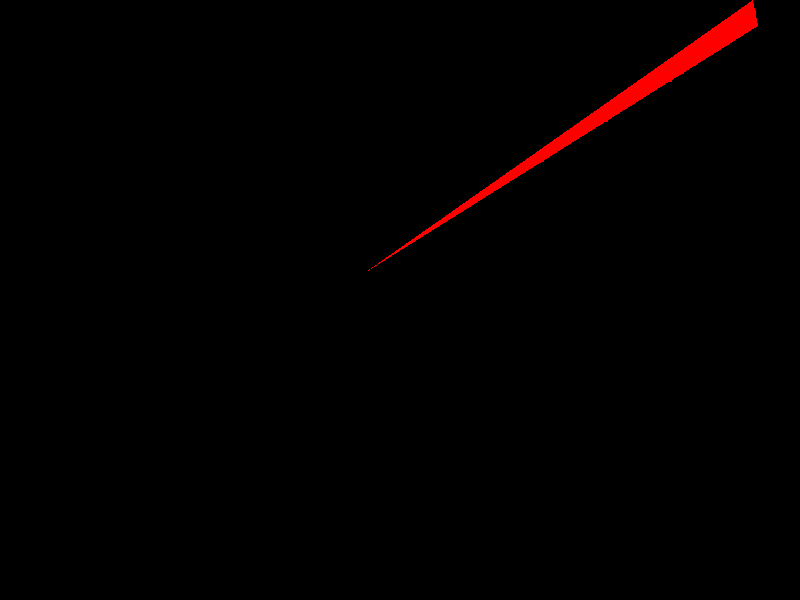
\includegraphics[width=.3\linewidth,bb = 0 0 30cm 30cm]{figure/Result7.png}
    }
    \subfloat{
        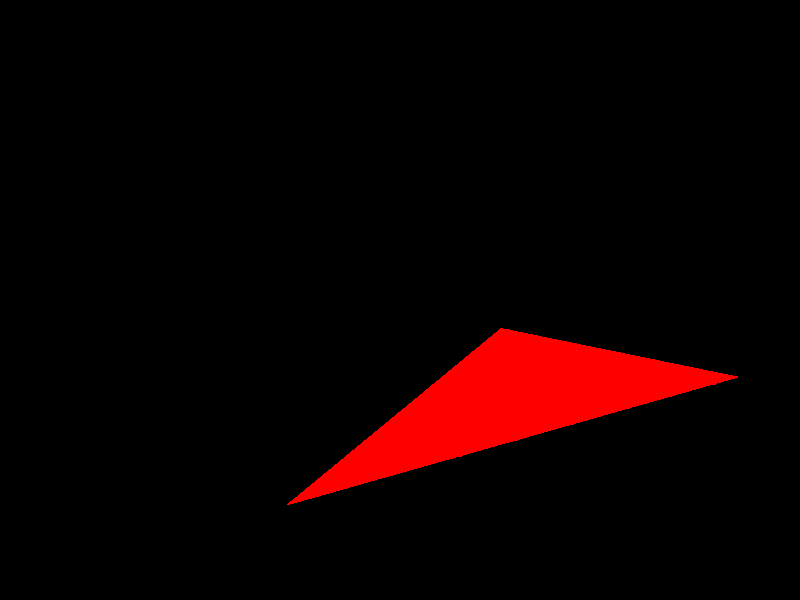
\includegraphics[width=.3\linewidth,bb = 0 0 30cm 30cm]{figure/Result8.png}
    }

    \caption{算法运行的测试结果}
    \label{fig:9 test results}
\end{figure}
本课题通过将将100个随机三角形测试数据集\ref{data:100 random triangles}(数据集中每一行中的六个数字依次是三角形中的三个点的x坐标和y坐标)中的三角形全部绘制出来进行正确性的验证,图\ref{fig:9 test results}是前九个三角形,限于篇幅原因,其他的三角形绘制结果会放在源码文件夹中与源码一并提交。



\subsection{不同参数配置下的性能测试}


测试集合仍然使用了100个随机三角形测试数据集\ref{data:100 random triangles},本课题测试了Tile Seeker用时在[3,8]区间内,Tile Dispatch用时在[1,8]区间内,Tile Decomposer Unit在[1,4]区间内,Tile Decomposer Unit数量在[1,16]区间内的性能测试, 测试的结果附于代码目录resource/Statistics.xlsx。

可以发现在不同的时钟参数配置下,Tile Decomposer Unit数量与流水线的总耗时关系是固定的,如图\ref{fig:unit count time clock}所示。

在原定配置参数下(tile seek用时三个周期,Tile Dispatch用时一个周期,Tile Decomposer Unit 用时一个周期)只改变Decomposer Unit数量的工作性能如表\ref{tab:3 1 1 config}。

\begin{table}
    \label{tab:3 1 1 config}
    \resizebox{\linewidth}{!}{
    \begin{tabular}{|ccccccc|}
        \hline
Decomposer Unit Count &  Total Cycles &  Tile Seeker Work Load &  Tile Dispatch Work Load &  Mean Tile Decomposer Unit Work Load &  Inside Tile Decomposer Work Load &  Min Tile Raster Work Load  \\ \hline
         1 & 169550 & 2 & 0 & 74 & 19 & 19 \\ \hline
         2 & 86355 & 4 & 0 & 93 & 39 & 37 \\ \hline
         3 & 61143 & 5 & 0 & 92 & 58 & 53 \\ \hline
         4 & 52997 & 6 & 1 & 79 & 68 & 61 \\ \hline
         5 & 50336 & 7 & 3 & 67 & 73 & 64 \\ \hline
         6 & 49405 & 7 & 5 & 57 & 75 & 65 \\ \hline
         7 & 49083 & 7 & 8 & 49 & 76 & 66 \\ \hline
         8 & 48636 & 7 & 10 & 43 & 77 & 66 \\ \hline
         9 & 48225 & 7 & 13 & 38 & 78 & 67 \\ \hline
        10 & 47901 & 7 & 14 & 35 & 79 & 67 \\ \hline
         11 & 47274 & 7 & 16 & 32 & 80 & 68 \\ \hline
        12 & 46768 & 7 & 16 & 30 & 81 & 69 \\ \hline
       13 & 46621 & 7 & 16 & 27 & 81 & 69 \\ \hline
       14 & 46424 & 7 & 16 & 25 & 82 & 69 \\ \hline
        15 & 46396 & 7 & 16 & 24 & 81 & 70 \\ \hline
        16 & 46421 & 7 & 16 & 22 & 82 & 70 \\ \hline     
    \end{tabular}}
\end{table}


 

\subsubsection{Decomposer Unit 数量的配置}
\begin{figure}[H]
    \centering
    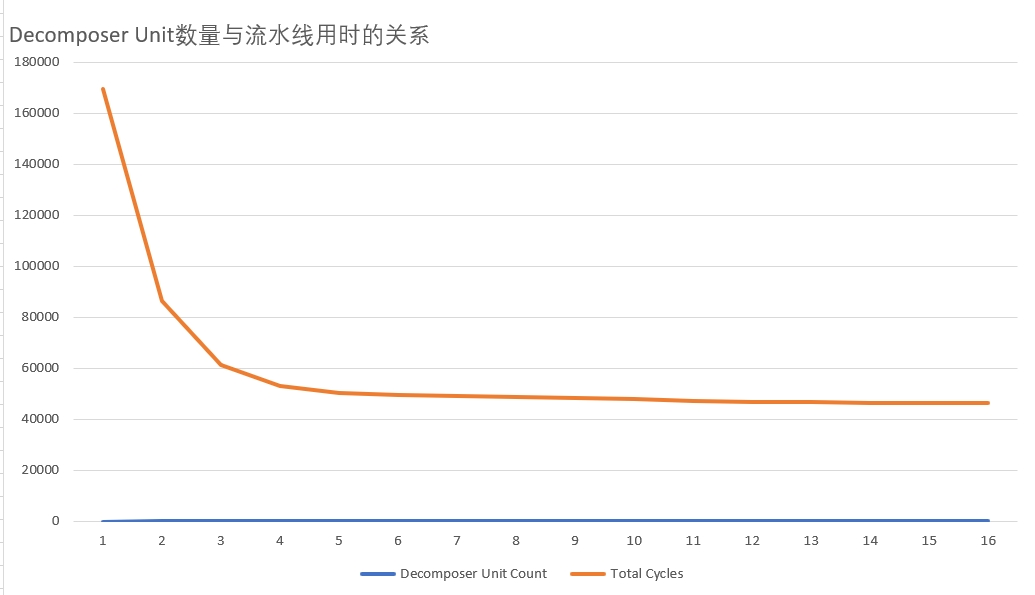
\includegraphics[width=.5\linewidth]{figure/plot1.png}
    \caption{不同Decomposer Unit数量情况下的流水线用时}
    \label{fig:unit count time clock}
\end{figure}   
考虑到Decomposer Unit在底层中的实现,本课题认为Decomposer Unit的数量应当是2的幂次,因而考虑图\ref{fig:unit count time clock}和表\ref{tab:3 1 1 config}, Decomposer Unit = 4是最能够充分利用Decomposer Unit且不影响下游流水线饱和工作的配置。

\subsubsection{时钟周期的配置}

流水线的工作性能除了取决于每个周期内流水线的并行工作量,也取决于流水线时钟的速率,如果要提升流水线的速率,我们的流水线的流水级数就要更高,也就是流水线每个阶段耗费时钟周期数量越长。
\begin{figure}[H]
    \centering
    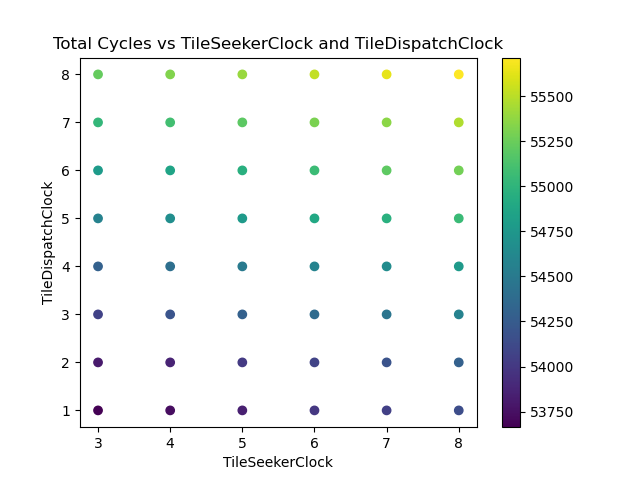
\includegraphics[width=.5\linewidth]{figure/plot2.png}
    \caption{\label{fig:2 clock change}流水线运行时间关于(TileSeekerClock,TileDispatchClock)的二元图像}
\end{figure}
表\ref{tab:fix decomposer}是Decomposer Unit数量为4,Tile Decomposer Unit固定为4时,改变TileSeekerClock和TileDispatchClock得到的测试数据,绘制图像如图\ref{fig:2 clock change}。可以看出,TileSeekerClock和TileDispatchClock的增加对流水线运行时长的影响较小,因此流水线的TileSeekerClock可以取8,TileDispatchClock可以取4。
\begin{table}[!ht]
    \centering
    \label{tab:fix decomposer}
    \resizebox{\linewidth}{!}{
    \begin{tabular}{|cccccccc|}
    \hline
        TileSeekerClock &  TileDispatchClock &  Total Cycles &  Tile Seeker Work Load &  Tile Dispatch Work Load &  Mean Tile Decomposer Unit Work Load &  Inside Tile Decomposer Work Load &  Min Tile Raster Work Load  \\ \hline
        3 & 1 & 53664 & 6 & 1 & 78 & 68 & 60 \\ \hline
        3 & 2 & 53801 & 6 & 1 & 78 & 67 & 60 \\ \hline
        3 & 3 & 54067 & 6 & 1 & 78 & 67 & 60 \\ \hline
        3 & 4 & 54294 & 6 & 1 & 77 & 67 & 59 \\ \hline
        3 & 5 & 54572 & 6 & 1 & 77 & 66 & 59 \\ \hline
        3 & 6 & 54777 & 6 & 1 & 77 & 66 & 59 \\ \hline
        3 & 7 & 55024 & 6 & 1 & 76 & 66 & 59 \\ \hline
        3 & 8 & 55229 & 6 & 1 & 76 & 66 & 58 \\ \hline
        4 & 1 & 53736 & 6 & 1 & 78 & 68 & 60 \\ \hline
        4 & 2 & 53858 & 6 & 1 & 78 & 67 & 60 \\ \hline
        4 & 3 & 54196 & 6 & 1 & 77 & 67 & 59 \\ \hline
        4 & 4 & 54408 & 6 & 1 & 77 & 67 & 59 \\ \hline
        4 & 5 & 54672 & 6 & 1 & 77 & 66 & 59 \\ \hline
        4 & 6 & 54859 & 6 & 1 & 77 & 66 & 59 \\ \hline
        4 & 7 & 55092 & 6 & 1 & 76 & 66 & 58 \\ \hline
        4 & 8 & 55323 & 6 & 1 & 76 & 66 & 58 \\ \hline
        5 & 1 & 53847 & 6 & 1 & 78 & 67 & 60 \\ \hline
        5 & 2 & 54010 & 6 & 1 & 78 & 67 & 60 \\ \hline
        5 & 3 & 54290 & 6 & 1 & 77 & 67 & 59 \\ \hline
        5 & 4 & 54497 & 6 & 1 & 77 & 67 & 59 \\ \hline
        5 & 5 & 54776 & 6 & 1 & 77 & 66 & 59 \\ \hline
        5 & 6 & 54956 & 6 & 1 & 76 & 66 & 59 \\ \hline
        5 & 7 & 55200 & 6 & 1 & 76 & 66 & 58 \\ \hline
        5 & 8 & 55394 & 6 & 1 & 76 & 65 & 58 \\ \hline
        6 & 1 & 53999 & 6 & 1 & 78 & 67 & 60 \\ \hline
        6 & 2 & 54073 & 6 & 1 & 78 & 67 & 60 \\ \hline
        6 & 3 & 54374 & 6 & 1 & 77 & 67 & 59 \\ \hline
        6 & 4 & 54578 & 6 & 1 & 77 & 66 & 59 \\ \hline
        6 & 5 & 54894 & 6 & 1 & 76 & 66 & 59 \\ \hline
        6 & 6 & 55059 & 6 & 1 & 76 & 66 & 59 \\ \hline
        6 & 7 & 55301 & 6 & 1 & 76 & 65 & 58 \\ \hline
        6 & 8 & 55523 & 6 & 1 & 76 & 65 & 58 \\ \hline
        7 & 1 & 54050 & 6 & 1 & 78 & 67 & 60 \\ \hline
        7 & 2 & 54185 & 6 & 1 & 77 & 67 & 59 \\ \hline
        7 & 3 & 54461 & 6 & 1 & 77 & 67 & 59 \\ \hline
        7 & 4 & 54654 & 6 & 1 & 77 & 66 & 59 \\ \hline
        7 & 5 & 54961 & 6 & 1 & 76 & 66 & 59 \\ \hline
        7 & 6 & 55205 & 6 & 1 & 76 & 66 & 58 \\ \hline
        7 & 7 & 55360 & 6 & 1 & 76 & 65 & 58 \\ \hline
        7 & 8 & 55637 & 6 & 1 & 75 & 65 & 58 \\ \hline
        8 & 1 & 54143 & 6 & 1 & 78 & 67 & 60 \\ \hline
        8 & 2 & 54292 & 6 & 1 & 77 & 67 & 59 \\ \hline
        8 & 3 & 54570 & 6 & 1 & 77 & 67 & 59 \\ \hline
        8 & 4 & 54770 & 6 & 1 & 77 & 66 & 59 \\ \hline
        8 & 5 & 55052 & 6 & 1 & 76 & 66 & 59 \\ \hline
        8 & 6 & 55276 & 6 & 1 & 76 & 66 & 58 \\ \hline
        8 & 7 & 55470 & 6 & 1 & 76 & 65 & 58 \\ \hline
        8 & 8 & 55713 & 6 & 1 & 75 & 65 & 58 \\ \hline
    \end{tabular}
    }
\end{table}




对TileSeekerClock和TileDispatchClock的讨论是建立在TileDecomposer = 4的情况下讨论的,TileDecomposerClock = 4的情况是对一个tile四个点的判断是串行的,如果要讨论TileDecomposerClock,可以讨论其取值为1,2,4, 当流水线的TileSeekerClock取8,TileDispatchClock取4时,流水线的的用时关于TileDecomposerClock的关系如表\ref{tab:change decompose clock}, 可以发现,TileDecomposerClock的增加对流水线用时的影响很小。

\begin{table}
    \centering
    \caption{TileDecomposerClock对流水线的影响}
    \label{tab:change decompose clock}
    \begin{tabularx}{\linewidth}{|XX|}
        \hline
        TileDecomposerClock &  Total Cycles \\ \hline
        1 & 53975 \\ \hline
        2 & 54195 \\ \hline
        4 & 54770 \\ \hline
    \end{tabularx}
\end{table}

根据Statistics.xlsx中的测试数据,我们可以发现,流水线对于TileSeekerClock,TileDispatchClock和TileDecomposerClock的时钟周期增加是不敏感的,这代表着我们可以通过进一步细化流水线来提高并行性能, 也就是说本课题提出的并行系统具有可延展性。
\subsection{缓冲区的大小}
参考\cite{CA}中的queuing theory,本课题认为缓冲区的长度应当满足Little's Law\ref{eq:Little's Law},其中$L,\lambda,W$分别指队列的长度,根据目前的系统参数配置(TileSeekerClock=8,TileDispatchClock=8,TileDecomposeClock=4,DecomposerUnitCount=4), 我们计算了各缓冲区的每周期平均到达的tile数量,tile在缓冲队列中的平均等待时间以及据此计算出的理想队列长度如表\ref{tab:queue length}。

\begin{table}[!ht]
    \centering
    \caption{系统中各缓冲区的理想长度计算}
    \label{tab:queue length}
    \begin{tabularx}{\linewidth}{|XXXX|}
    \hline
        Quene &  $\lambda$ &  W & L \\ \hline
        x32TileFifo & 0.0537 & 2.39 & 1 \\ \hline
        x16TileFifo & 0.11 & 5.84 & 1 \\ \hline
        x8TileFifo & 0.11 & 4.39 & 1 \\ \hline
        x4TileFifo & 0.11 & 2.65 & 1 \\ \hline
        x2TileFifo & 0.11 & 8.67 & 1 \\ \hline
        DecomposerUnit0 & 0.208 & 10.7 & 0 \\ \hline
        DecomposerUnit1 & 0.197 & 10.7 & 0 \\ \hline
        DecomposerUnit2 & 0.19 & 10.6 & 0 \\ \hline
        DecomposerUnit3 & 0.185 & 10.6 & 0 \\ \hline
        InsideTileFifo & 0.823 & 101 & 83 \\ \hline
        InsideMaskFifo & 9.18 & 1.06 & 10 \\ \hline
        RasterMaskFifo & 0.6 & 1.06 & 1 \\ \hline
    \end{tabularx}
\end{table}


\subsection{与串行系统的对比}

串行系统判断点在三角形内的方式是对三角形bounding box内的像素逐一检查,100个随机三角形测试数据集中的三角形bounding box中的像素和为7830343,相比于我们前面使用的TileSeekerClock=8,TileDispatchClock=8,TileDecomposeClock=4,DecomposerUnitCount=4的配置下54770的运行周期,串行系统若每周期判断142个像素才能达到本课题提出的并行系统的性能,但这样做的硬件成本已经远远超过了我们的并行系统。
我们的并行系统等价于每周期能够并行判断4到8个像素(DecomposerUnit中每周期判断子tile的一个顶点,TileSeeker中需要判断当前tile以及相邻tile),串行系统每周期判断8个像素所用周期为978792, 我们的并行系统的用时仅为串行系统的5.6\%。

\subsection{与naive并行系统的对比}

这里的对比是我们相对于原始的四级流水TileDecomposer的性能对比。

\begin{table}
    \caption{\label{tab:current system}目前设计下100个随机三角形下的算法系统负载}

    \begin{tabularx}{\linewidth}{|XXX|}
        \hline
        模块 & 运行周期 & 负载率(\%) \\ \hline
        所有模块 & 55173 & 100 \\ \hline
        TileSeeker & 3342 & 6  \\ \hline
        TileDispatch & 551 & 1 \\ hline
        DecomposerUnit(Mean) & 41380 & 75  \\ \hline
        Inside Tile Decomposer & 35862 & 65 \\ \hline
        Minumum Tile Raster & 32000 & 58 \\ \hline
    \end{tabularx}
\end{table}


\begin{table}
    \caption{\label{tab:naive system}四级流水系统下100个随机三角形下的算法系统负载}
    \begin{tabularx}{\linewidth}{|XXX|}
        \hline
        模块 & 运行周期 & 负载率(\%) \\ \hline
        所有模块 & 49063 & 100 \\ \hline
        Tile Seeker & 3645 & 5.2  \\ \hline
        Tile Decomposer 32 & 2910 & 4.1  \\ \hline
        Tile Decomposer 16 & 5953 & 8.4  \\ \hline
        Tile Decomposer 8 & 11828 & 17  \\ \hline
        Tile Decomposer 4 & 21553 & 31  \\ \hline
        Inside Tile Decomposer & 37789 & 77 \\ \hline
        Minumum Tile Raster & 32496 & 66 \\ \hline
    \end{tabularx}
\end{table}

原始的并行系统设计和目前的并行系统设计的各模块运行数据分别如表\ref{tab:naive system}和表\ref{tab:current system}, 虽然目前的流水线设计比原设计慢了12\%,但是在如下两点拥有优越性。

\begin{enumerate}
    \item \textbf{冗余计算单元}:目前系统设计的冗余计算单元较少,各个模块的负载率保持在合理区间,原系统的设计中明显可以看出各级Decomposer存在严重的计算单元冗余问题,负载率较低,硬件成本较高。
    \item \textbf{流水线细分程度更高}:目前系统设计采用的时钟参数配置为TileSeekerClock=8,TileDispatchClock=8,TileDecomposeClock=4,DecomposerUnitCount=4,相比于原系统的TileSeekerClock=3,TileDecomposeClock=1,目前的设计显然更能接受更细分的流水线设计,拥有更高的性能提升空间。
\end{enumerate}